\documentclass[pucformat]{XPucThesis}
\usepackage{fixltx2e}
\usepackage[utf8]{inputenc}
\usepackage{times}
\usepackage{setspace}
\usepackage{ifthen}
\usepackage{lscape}
\usepackage{amsmath,amssymb,amsbsy,amsfonts}
\usepackage{mathrsfs}
\usepackage{fancyhdr}
\usepackage{float}
\usepackage{subfig}
\usepackage{rotating}
\usepackage{pdfpages}
\usepackage{color}
\usepackage{ifpdf}             
\usepackage{array}
\usepackage{sistyle}
\usepackage{nicefrac}
\usepackage{longtable}  
\usepackage[stable]{footmisc}    
\usepackage{wasysym}

% Graphics packages for dual use of LaTeX and pdfTeX and other graphics handling definitions.
\ifpdf
 \usepackage[pdftex]{graphicx}
 \usepackage{epstopdf}
 \DeclareGraphicsExtensions{.eps,.jpg,.png,.pdf}
 \graphicspath{{\figpath}}
\else
 \usepackage[dvips]{graphicx}
 \DeclareGraphicsExtensions{.eps}
 \graphicspath{{\figpath}}
\fi

\usepackage[bookmarks=true,pdftex]{hyperref}
\hypersetup{%
    colorlinks=true,
    linkcolor=black,
    citecolor=black,
    urlcolor=black,
    filecolor=black,
    plainpages=false,
    pdftitle={},
    pdfauthor={Nombre},
    pdfsubject={T\'itulo},
    pdfkeywords={Palabras clave},
    pdfproducer=PDFLaTeX,
    pdfstartview=FitH,
    pdfpagemode=UseOutlines,
    bookmarksopen=true,
    bookmarksopenlevel=0,
    verbose=true
}
%\usepackage[natbibapa]{apacite}
\usepackage[]{apacite}

% List used files in logfile
\listfiles

% New Theorem-based environments names
\newtheorem{definition}{\bf Definition}[chapter]
\newtheorem{property}{Property}[chapter]
\newtheorem{claim}{Claim}[chapter]
\newtheorem{lemma}{\bf Lemma}[chapter]
\newtheorem{proposition}{Proposition}[chapter]
\newtheorem{theorem}{\noindent \bf Theorem}[chapter]
\newtheorem{corollary}{\bf Corollary}[chapter]
\newtheorem{pf}{Proof}[chapter]
\newtheorem{example}{\bf Example}[chapter]
\newtheorem{remark}{Remark}[chapter]

% Filepath definitions
\newcommand{\latexroot}{.}
\newcommand{\defpath}{\latexroot/def}
\newcommand{\bibpath}{.}
\newcommand{\figpath}{./figs}	
\newcommand{\textpath}{./text}
\newcommand{\paperloc}{papers}

% Define references names
\newcommand*{\figref}[1]{\figurename~\ref{#1}}
\newcommand*{\tableref}[1]{\tablename~\ref{#1}}
\newcommand*{\chapref}[1]{Cap\'itulo~\ref{#1}}
\newcommand*{\secref}[1]{Secci\'on~\ref{#1}}
\newcommand*{\eqnref}[1]{Ecuaci\'on~(\ref{#1})}

% Redefine styles
\renewcommand{\thesubfigure}{\textsc{\alph{subfigure}}} 


% Figure shortcuts
\newcommand{\fig}[4]{
  \begin{figure}[ht]	
    \centering
    \fbox{\resizebox{#3}{!}{\includegraphics{\figpath/#2}}}
    \caption{#4}
    \label{#1}
  \end{figure}
\normalsize
}
\newcommand{\sfig}[8]{
  \begin{figure}[ht]	
    \centering%
    \subfloat[][]{\label{#3}%
    		\fbox{\resizebox{#4}{!}{\includegraphics{\figpath/#2}}}}\qquad%
    \subfloat[][]{\label{#6}%
    		\fbox{\resizebox{#7}{!}{\includegraphics{\figpath/#5}}}}%
    \caption{#8}%
    \label{#1}%
  \end{figure}
\normalsize
}

\begin{document}

\mdate{December XX, 2013}
\version{\today}

\title[TITLE]{\textbf{Discrete-time noise filtering for Pulse-Processing in Particle Physics Experiments}}
\author[AUTOR]{Diego Ávila Gárate}
\address{Escuela de Ingenier\'ia\\
         Pontificia Universidad Cat\'olica de Chile\\ 
         Vicu\~na Mackenna 4860\\
         Santiago, Chile\\
         {\it Tel.\/} : 56 (2) 354-2000}
\email{dlavila@uc.cl}

\facultyto    {the School of Engineering}
\faculty      {Faculty of Engineering}
\degree       {Master of Science in Engineering} 
\advisorA{Ángel Abusleme Hoffman} 
\advisorB{} % de existir, segundo supervisor

% Committee
\committeememberA{Marcelo Guarini Herrmann}
\guestmemberA{Pablo Zegers Fernández}
\ogrsmember{Jaime Navón Cohen}

% Subject
\subject{Engineering}

% Date
\date{July 2014} %FECHA

% Copyright
\copyrightname{Diego Ávila Gárate} %AUTOR
\copyrightyear{MMXIV} %AÑO

% Dedication
\dedication{\mbox{}}

% Preliminaries: cover page and dedication
\NoChapterPageNumber    % no header - footer on first page of chapter
\pagenumbering{roman}

% Make title
\maketitle

\cleardoublepage

%%%%%%%%%%%%%%%%%%%%%%%%%%%%%%%%%%%%%%%%%%%%%%%%%%%%%%%%%%%%%%%%%%%%%%%%
% Acknowledgements

\chapter*{ACKNOWLEDGEMENTS}

First and foremost I'd like to thank my advisor, Professor Ángel Abusleme, whose enthusiasm, patience, and knowledge, were fundamental to achieve the most precious goal of any grad student, reach the end of his thesis. I promise you that someday we'll have a quadcopter battle.

I wish to thank to all those who are and were members of the IC-UC group, and especially to Professor Enrique Álvarez, Hernán Campillo and Cristóbal Alessandri.

I would like to express my gratitude to Cleve Moler, for making such a terrific piece of software call \textsc{Matlab}, which was a fundamental tool for the development of this thesis. I am also extremely grateful to Donald Knuth and Leslie Lamport.

Finally, I want to thank to my family for the continuous love they have provided me through my entire life.


\cleardoublepage


\tableofcontents
\listoffigures
\listoftables

\cleardoublepage

\MScAbstract{Particle Physics is the branch of physics that studies the fundamental constituents of matter and radiation, and their mutual interactions. The main tools used by particle physicists are particle accelerators, which use electromagnetic fields to accelerate charged particles to relativistic speeds before they are made to collide inside detectors. The International Linear Collider (ILC), a next generation, 31-kilometer long linear particle accelerator, will smash electron and positron bunches at up to 500 GeV. Located at the ILC detector forward region is the BeamCal, a highly segmented calorimeter detector. The BeamCal specifications for radiation tolerance, noise, signal charge, pulse rate and occupancy pose unique challenges for the instrumentation system.

Framed in the design, integration and testing of the Bean IC, a 5-channel application specific integrated circuit (\textsc{asic}) planned to meet the BeamCal instrumentation needs, this thesis presents: the development of a new mathematical framework for a design-oriented analysis of discrete-time filters in the discrete-time domain; and the design and implementation of a switched-capacitor (SC) filter for arbitrary weighting function synthesis to be included in the Bean IC, which aims to take full advantage of the introduced mathematical framework. 

}{Charge Measurements, Low-noise filters, Noise, Nuclear Physics Instrumentation, Optimum Digital Filtering.}

\cleardoublepage

\MScResumen{
La Física de Partículas es la rama de la física que estudia las constituyentes fundamentales de la materia y la radiación, y sus interacciones mutuas. Las principales herramientas utilizadas por los físicos de partículas son los aceleradores de partículas, los cuales usan campos electromagnéticos para acelerar partículas cargadas a velocidades relativistas, para después hacerlas colisionar dentro de detectores. El Colisionador Lineal Internacional (ILC) es un acelerador de partículas lineal de la próxima generación de 31 kilómetros de largo que colisionará grupos de electrones y positrones a 500 GeV. Ubicado en la región delantera del ILC se encuentra el BeamCal, un calorímetro altamente segmentado. Las especificaciones del BeamCal para tolerancia a la radiación, ruido, señal de carga, tasa de pulsos y ocupación plantean desafíos únicos para el sistema de instrumentación.

Enmarcado en el diseño, integración y prueba de \emph{Bean IC}, un circuito integrado de aplicación específica (\textsc{asic}, por su sigla en inglés) de cinco canales para satisfacer las necesidades de instrumentación del BeamCal, esta tesis presenta: el desarrollo de un nuevo marco matemático para el análisis orientado al diseño de filtros de tiempo discreto; y el diseño y implementación de un filtro de capacitores conmutados para la síntesis de funciones de peso arbitraria que será incluido en \emph{Bean IC}, el cual busca aprovechar al máximo el marco matemático propuesto.


}{Medición de carga, Filtros de Bajo Ruido, Ruido, Instrumentación para Física Nuclear, Filtrado Digital Optimo.}

\cleardoublepage
\pagenumbering{arabic}
\setlength{\labelsep}{1em}

\newcommand\blfootnote[1]{%
  \begingroup
  \renewcommand\thefootnote{}\footnote{#1}%
  \addtocounter{footnote}{-1}%
  \endgroup
}

\chapter{INTRODUCCIÓN}
\label{chapter:introduction}
\section{Experimentos de física de partículas}
\blfootnote{Esta memoria fue financiada por la Comisión Nacional para la Investigación Científica y Tecnológica (CONICYT) de Chile, en virtud de la concesión del fondo FONDECYT  11110165.} 


	La física de partículas es una rama de la física que estudia la naturaleza de las partículas fundamentales que constituyen la materia y la radiación \citep{wiki}. El estudio de las partículas elementales ha permitido a la humanidad responder algunas de las preguntas más profundas de la físicas, lo cual ha impactado en nuestras vidas a diferentes escalas, desde avances en la comprensión del universo, la composición de la materia y la existencia de nuevas dimensiones, hasta aplicaciones en el desarrollo de tecnologías de uso cotidiano. 

	La principal herramienta utilizada en la física de partículas son los aceleradores de partículas. El principio básico de un acelerador consiste en concentrar partículas subatómicas en un haz y luego acelerarlas a velocidades cercanas a la velocidad de la luz por medio de campos electromagnéticos. Posteriormente, estos haces se hacen colisionar dentro de un detector, ya sea contra objetivos estacionarios u otro haz de partículas viajando en la dirección opuesta.  Como resultados de estas colisiones, se liberan subproductos que son dispersados desde el punto de la colisión. Los detectores se encuentran compuestos por cientos de sensores que permiten medir distintos fenómenos a partir de las colisiones. El estudio y posterior procesamiento de los datos recopilados  provee a los científicos información sobre la naturaleza de las partículas elementales.

	Para realizar las colisiones entre partículas, es necesario alcanzar altos niveles de energía cinética. Debido a que los aceleradores deben trabajar a estas grandes escalas de energía, la física de partículas también recibe el nombre de "física de altas energías".  La nueva generación de instrumentos pretende trabajar en escalas de energía nunca antes utilizadas, denominada "escala tera" (1TeV), la cual permitirá replicar niveles de energía solo alcanzados en los orígenes del universo. En la actualidad se encuentran en curso dos proyectos que pretenden abrir las puertas a un nuevo mundo de investigación denominado el universo cuántico \citep{ilc101}: \textit{El Gran Colisionador de Hadrones} (LHC; Large Hadron Collider), desarrollado por la Organización Europea de Investigación Nuclear (CERN) actualmente en etapa de actualización. Y el \textit{Colisionador Lineal Internacional} (ILC; International Lineal Collider), un colisionador aun en desarrollo, pensado para estar operativo entre el 2010 - 2020, a cargo de esfuerzos conjuntos de diversos países coordinados mediante el \textit{Global Design Effort} (GDE) y el \textit{World Wide Study}.
 Se espera que la combinación de ambos aceleradores conducirán a grandes descubrimientos para la humanidad, como fue la confirmación de la existencia del campo de Higgs en esta década gracias al LHC, considerado uno de los logros más grandes de la ciencia del último medio siglo al contribuir a completar el modelo estándar.

	Con niveles de energía cada vez más altos y sistemas de detección cada vez más precisos, la construcción de un acelerador representa un desafío de elevada complejidad. Para alcanzar dichos objetivos, son necesarias construcciones de algunas decenas de kilómetros de radio y esfuerzos colaborativos internacionales que involucran a cientos de científicos e ingenieros a lo largo de todo el mundo. Es por esta razón que los aceleradores son considerados como la obras de ingeniería más grandes y ambiciosas jamás construidas por la humanidad.

	A su vez, la elevada complejidad que implica el desarrollo de un acelerador de partículas,  demanda el desarrollo de tecnologías en el estado del arte y representa una enorme y continua fuente de retos y desafíos, la cual a llamado la atención de la comunidad científica durante las ultimas décadas.  Los conocimientos obtenidos en la búsqueda de soluciones para estos desafíos, han ayudado a gran y pequeña escala en mejorar la calidad de vida de los humanos. Ejemplos concretos son la creación del internet, la cual fue desarrollada por el CERN como un proyecto para satisfacer la necesidad de compartir grandes cantidades de información entre distintos centros de investigación. O la creación de los syncotrones, los cuales utilizan un principio muy similar a los aceleradores para generar radiación y son utilizados en la medicina moderna tanto para estudiar enfermedades como para desarrollar medicamentos para combatirlas \citep{tuttle101}.

Esta tesis de pregrado trata sobre el diseño y la implementación de una plataforma de pruebas para el estudio y  la caracterización de un circuito integrado destinado a implementar los resultados expuestos en \citep{diegothesis} que forman parte de el trabajo colaborativo para desarrollar nuevas tecnologías que permitan mejorar el desempeño de la obtención de datos en los detectores, disminuyendo los efectos del ruido presente en la electrónica de \textit{front-end}.

\section{Electrónica en detectores de partículas}

	 Un detector en física de partículas es un sistema dedicado a recolectar las pistas sobre la identidad de las partículas (como su masa, velocidad, carga entre otras propiedades) a partir de los distintos fenómenos sensables posterior a una colisión. Comúnmente son tres los tipos de detectores utilizados en física de partícula: Los detectores de trayectoria, los cuales se encargan de reconstruir la trayectoria que dejan las partículas luego de una colisión (principalmente partículas que reaccionan poco con la materia como los muones o los neutrinos); los calorímetros, los cuales se encargan de medir la cantidad de energía al detener y absorber la energía de las partículas; y los detectores identificadores de partículas, los cuales se encargan de determinar la identidad de las partículas midiendo alguna propiedad específica (como la radiación de Cherenkov) o infiriéndola de balances respecto a otras mediciones \citep{cern101}.

	En la actualidad los detectores de partículas presentes en los colisionadores representan  grandes cámaras, comúnmente de forma cilíndrica coaxiales al eje de movimiento del haz de partículas, en donde se llevan a cabo las colisiones. Estos detectores de partículas se encuentran compuestos por capas de subdetectores, en donde cada capa tiene por objetivo obtener información de algún fenómeno específico. Cada una de estas capas se encuentra altamente segmentada por múltiples detectores que forman una unidad básica de detección (o pixel), permitiendo una mejor resolución espacial de las mediciones. Cada unidades básicas de detector en conjunto con su respectiva electrónica (o \textit{front-end} del detector), conforman un canal. La estructura general de un canal esta constituida por: un detector, un pre amplificador, un filtro, un conversor análogo digital \citep{spieler2005semiconductor}. La figura XX muestra un esquema altamente simplificado de un canal de un detector.

	La necesidad de generar continuamente sistemas de detección más complejos con mayor desempeño y mayor precisión, han motivado a grandes equipos de colaboración internacional para desarrollar nuevas tecnologías cada vez más avanzadas que permitan alcanzar los estándares requeridos. En el campo de la electrónica se desarrollan continuos esfuerzos para mejorar el desempeño de los sistemas involucrados en la detección: Reducción de componentes, ahorro de energía, minimización de ruido, aumento de ancho de banda, son algunos de los aspectos que encaminan nuevas investigaciones.
	
	
%%hasta aca vamos bien
%%OJOOOOO REVISAR EL SIGUIENTE PARRAFO!!
	En este contexto, la minimización del ruido representa en la actualidad uno de los limites fundamentales para la resolución de las mediciones. Diversas investigaciones se han llevado a cabo para contribuir al entendimiento y el desarrollo de una estrategia de mitigación de este problema. Uno de los resultados que motiva el desarrollo de la presente tesis de pregrado fue presentado en \citep{avila101}. En este, se propone una nueva metodología de análisis de ruido  en el dominio discreto del tiempo para el diseño de filtros discretos. Esta metodología representa una importante herramienta de diseño para la electrónica de física de partículas y el análisis de ruido en general. \footnote{Un ejemplo particular de otra aplicación de esta herramienta,  lo representa el diseño de filtros para el \textit{front-end} de lectura de un CCD, en donde el ruido de lectura es crítico en la calidad de las imágenes obtenidas \citep{guzman101}}

	Con el motivo de llevar a la práctica los resultados presentados, se propone en \citep{diegothesis} el diseño de un ASIC que implementa un prototipo para la segunda iteración de the bean, denominado the bean v2. Este integrado consiste en la implementación un \textit{front-end} de 32 canales para ser utilizado en the BeamCal un detector destinado a formar parte del ILC. Una de las principales características de The bean v2, es que implementa la etapa del filtro de la figura XX por medio de un integrador diferencial de capacitores conmutados con ganancia configurable digitalmente, permitiendo de este modo generar un filtro discreto configurable.
 

\section{Experimentos y adquisición de datos en física de partículas}

Una de las características interesantes de la física de partículas es el hecho de que las herramientas necesarias para lograr los objetivos propuestos, en la mayoría de los casos, aun no han sido creadas. Debido a que cada nuevo instrumento representa en si mismo un conjunto de desafíos únicos, es necesario desarrollar herramientas que permitan estar a la altura. De este modo, las necesidades por parte de la instrumentación de experimentos ha impulsado los limites de la ciencia y la tecnología en muchos aspectos y, a su vez, nuevos desarrollos en la instrumentación a menudo son posible gracias a los avances en la tecnología.  En este sentido, los experimentos en la física de partícula y la tecnología son dependientes el uno del otro. \citep{Attila}

La inagotable oferta de desafíos llama continuamente a  cientos de científicos a proponer y desarrollar nuevas teorías y prototipos hasta poder desarrollar en conjunto una solución adecuada. Sin embargo, la especificidad y complejidad de estas soluciones comúnmente implican un alto costo de desarrollo tanto en recursos humanos, de tiempo y  monetarios. 
Incluso el desarrollo de prototipos demanda la implementación de complejos sistemas que permitan recrear condiciones existentes en los aceleradores para someter a pruebas las soluciones propuestas.

En el contexto de la electrónica, el esquema general de los sistemas de experimentos de física de partículas consiste en un detector o sensor, una etapa de \textit{front-end}, una etapa dedicada a la adquisición de los datos, un sistema de alimentación, un bloque de \textit{triggers} o generador de impulsos para estimular el sistema y por último un sistema de control el cual comúnmente lleva a cabo las tareas de sincronización del resto de los bloques y la interfaz de comunicación. En la figura XX se presenta un diagrama simplificado de la estructura general de un sistema de adquisición de datos.

	Gracias a las tecnologías de fabricación disponible, una de las opciones más populares en la actualidad consiste en implementar las distintas etapas (o varias de ellas) en un ASCI. Estos presentan grandes ventajas ya que integran múltiples funciones en un mismo \textit{chip}, entregando la posibilidad incluso de repetir dichas funciones dentro de un mismo integrado para  lidiar con la alta segmentación actual de los detectores, procesando varios canales a la vez. Sin embargo, pese a que los ASIC poseen bajos costos cuando se producen en masa, poseen un alto costo de fabricación y altos tiempos de manufactura y diseño. 
	
	Otra alternativa la representan las FPGA o Arreglos de compuertas de campo programable (Field programmable Gate Arrays), las cuales son una opción muy adecuadas para experimentos en física de partículas,  debido a su alto desempeño, amplia versatilidad, sus capacidades de procesamiento de señales, ancho de banda y programabilidad. Debido a que poseen una gran cantidad de  compuertas lógicas programables, las FPGA permiten implementar nuevos diseños digitales por un bajo costo y en cortos tiempos, con la posibilidad de implementar casi cualquier aplicación especifica, a su vez permiten corregir cualquier error de diseño simplemente cargando un nuevo firmware en el dispositivo. \citep{1644925,6341473,4669290}

Como es común en este tipo de situaciones, la soluciones mas adecuadas contemplan una combinación lineal de ambas alternativas, de este modo, es posible obtener una solución que aproveche las ventajas de tanto de los ASI como de las FPGA. Es por eso que en el campo experimental de la física de partículas es posible encontrar sistemas híbridos, o incluso ASI que integren procesamiento digital.



\section{Contenido de esta tesis}
El capítulo 2 comienza con una introducción al proyecto que inspira el trabajo presentado en esta memoria, el desarrollo de una plataforma de pruebas para la segunda iteración de the Bean, un circuito integrado de aplicación especifica (ASIC, por sus siglas en inglés) el cual forma parte de una propuesta para el ILC. A continuación se presentan los principales desafíos de este trabajo, haciendo hincapié en cada una de las limitantes y requisitos necesarios. En el capítulo 3 se presenta un detalle del prototipo de the Bean V2, tanto sus especificaciones físicas como un detalle de sus especificaciones funcionales. Junto con lo anterior, se entrega el diseño de las principales pruebas a considerar con el fin de corroborar el correcto funcionamiento del integrado. En el capítulo 4 se presenta un detalle de la plataforma implementada, especificando como fueron abordados cada uno de los requerimientos estipulados en el capítulo 2. También se entregan los \textit{layout} finales desarrollados en el software EAGLE y la metodología utilizada para implementar una comunicación \textit{on line} con un computador. En el capitulo 5 se presentan los resultados obtenidos analizando el resultado de la plataforma desarrollada, del software implementado y los principales resultados de la implementación de la plataforma así como los resultados de las pruebas realizadas a the Bean V2. Finalmente, en el capítulo 6 se entregan las principales conclusiones de este trabajo, analizando los resultados y la contribución de este trabajo y se presentan ideas para futuras contribuciones.  
\clearpage
\chapter{DEFINICIÓN DEL PROBLEMA}
\label{chapter:problem}
\hyphenation{BeamCal}
En esta tesis de pre-grado se describe el diseño y la implementación de una plataforma de pruebas cuyo fin es someter a pruebas y caracterizar un prototipo de the bean V2. Este es un ASCI diseñado para satisfacer necesidades de instrumentación del BeamCal, un detector del International Linear Collider.

\section{El colisionador lineal internacional}
El ILC es un colisionador de partículas aún  en etapa de diseño, que pretende complementar los descubrimientos realizados por el LHC en el 2012. Este instrumento colisionará electrones contra sus  anti-partículas los positrones, para lo cual cuenta principalmente de dos aceleradores los que comprenden una extension de aproximadamente 31 kilómetros. En estos aceleradores las partículas confinadas dentro de un haz son aceleradas por medio de campos electromagnéticos hasta alcanzar velocidades relativas a la velocidad de la luz, para luego ser colisionadas. La escala de energía en estas colisiones serán del orden de 500 GeV para su primera etapa. Posteriormente en una segunda etapa, el ILC contempla actualización que pretende utilizar una estructura de aceleradores de 50 kilómetros y niveles de energía de 1 Tev. Estos representan niveles de energía nunca antes observados en la tierra, es por esta razón que estos aceleradores reciben el nombre de aceleradores de ``escala tera". 

El proyecto del ILC representa un desafío de carácter mundial. Más de 300 laboratorios y Universidades de todo el mundo participan en el diseño de este nuevo instrumento de alto nivel para la física de partículas.  Debido a que tanto la realización de un proyecto de esta magnitud, así como las tareas de coordinación representan un desafío extremadamente complejo, muchas de las especificaciones que comprenden al proyecto aun están en discusión. Un ejemplo de esto es el emplazamiento de este proyecto, el cual aun no se encuentra definido.


\section{El detector frontal y the BeamCal}
	En un acelerador de partículas las colisiones se llevan a cabo dentro de un gran detector, el cual esta a su vez compuestos de un conjunto de distintos detectores, destinados a medir fenómenos específicos. La estructura de estos detectores para el ILC aun permanece en estudio, sin embargo, existen dos propuestas validadas como candidatas. Cada una de estas propuestas considera la presencia de un detector frontal en su estructura. El propósito de este detector frontal es realizar mediciones de la luminosidad de alta velocidad y precisión, y asegurar la hermiticidad del detector.
	Para lograr dichas tareas, el detector frontal cuenta a su vez con dos calorímetros principales ubicados en las capas más cercanas al haz de partículas: el LumiCal y el BeamCal.
The BeamCal es un calorímetro electromagnético altamente segmentado,  adyacente al haz de partículas y cuenta principalmente con tres propósitos: Mejorar la hermeticidad del ILC para ángulos polares bajos, reducir el backscattering para pares en la parte interior del detector del ILC y asistir al diagnostico del haz de partículas. Las especificaciones del BeamCal para la tolerancia de radiación, ruido, carga de señal, tasas de pulsos y tiempos de ocupación plantean un reto único para el sistema de instrumentación. 

\section{The bean V2}
The bean V2 es un IC que implementa la segunda iteración de The bean. Este integrado tiene como objetivo implementar el  front-end para un detector destinado a formar parte de BeamCal. En su segunda iteración The bean V2 contempla integrar la electronica para 32 canales. Cada uno de estos canales contará con: un amplificador sensible a la carga (CSA), con un pulsador de pre-carga; un filtro de capacitores conmutados (SC) totalmente diferencial con características de supresión de bajo ruido; un conversor análogo-digital(ADC) totalmente diferencial de aproximación sucesiva de 10 bits; y sistema para almacenar la información de salida, ya sea en una memoria analógica o digital. Adicionálmente, el IC cuenta con una red de feed-back para propósitos de diagnostico. En la figura \ref{fig:thebean_diagram} se entrega un diagrama de la estructura de The bean. 
  
\begin{figure}[!t]
	\centering
	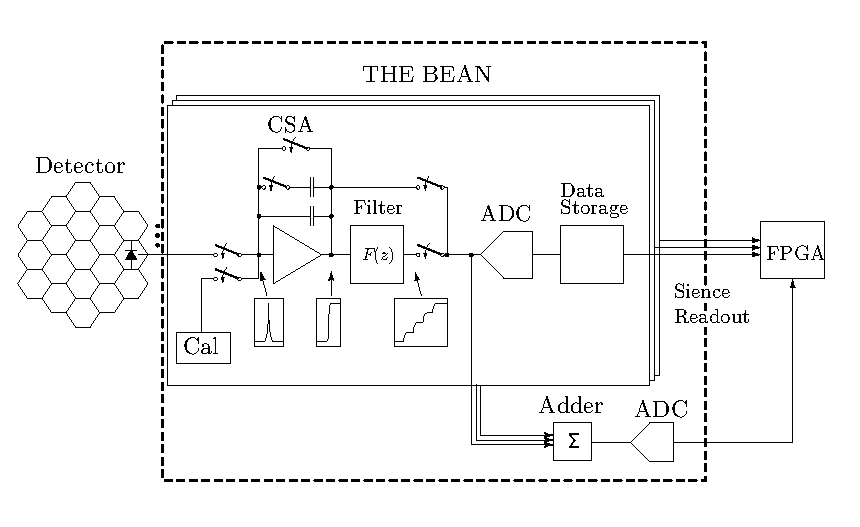
\includegraphics[width=5in]{./figures/thebeamdiagram-02.eps}
	\caption{Diagrama de bloques de The bean.}\label{fig:thebean_diagram}
\end{figure}
 
El IC debe ser capaz de procesar la información proveniente del detector BeamCal a una frecuencia nominal de 3.2468 MHz, con un 100\% de ocupación. Por otro lado, debe ser capaz de lidiar con dos modos diferentes de operación: El modo de adquisición estandar (standar data taking mode o SDT mode) y el modo de calibración del detector (Detector Calibration mode o DCal mode). Según las especificaciones de BeamCal, la máxima señal de entrada corresponde aproximadamente a $37pC$ en el modo SDT  y 50 veces menor en el modo DCal.
Por otro lado, dada la proximidad del detector a las colisiones, se encontrará expuesto a granes cantidades de radiación (1Mrad $\text{SiO}_2$).

\begin{table}[!h]
	\begin{center}
		\begin{tabular}{|l|l|}\hline
			Tasa de entrada & $3.25\,\text{MHz}$ durante $0.87\,\text{ms}$, repetidos cada $200\,\text{ms}$ \\ \hline
			Canales por AISC & $32$ \\ \hline
			Ocupación & $100\%$ \\ \hline
			Resolución & $10$ bits por un canal individual, $8$ bits para la cadena de \textit{fast feedback} \\ \hline
			Modos de Operación & Modo de adquisición estandar (STD), Modo de calibración del detector (DCal) \\ \hline
			Señal de entrada & Hasta $40$ pC en el modo SDT, $0.74$ pC en el modo DCal \\ \hline
			Capacitancia de entrada & $65$ pF \\ \hline
			Características adicionales  & Baja latencia de salida($1\,\micro\text{s}$)\\ \hline
			Características adicionales  & Pulsador interno para calibración electrónica\\ \hline
			Tolerancia de radiación & 1 Mrad ($\text{SiO}_2$),TID \\ \hline
			Consumo & $2.19$ mW  por canal \\ \hline
			\end{tabular}
		\vspace*{5pt}
		\caption{Resumen de las especificaciones para el ASIC de instrumentación para the BeamCal.}\label{tab:bean_specs}
	\end{center}
\end{table}

 La tabla \ref{tab:bean_specs} resume las especificaciones a las que se encontrará sometido el IC The bean V2, las cuales son heredadas de los requisitos exigidos por the BeamCal.
 
\section{La plataforma de pruebas}
	El desafío del trabajo presentado en esta tesis de pre-grado consiste en lograr implementar una plataforma que permita instanciar todas las condiciones necesarias para probar el funcionamiento de un  prototipo para the bean V2 \citep{diegothesis}. En la figura \ref{fig:thebean_spec} se presenta la estructura general de las señales que intervienen en el IC. Esta investigación se realizó bajo el patrocinio de CONICYT a través del programa FONDECYT.
El FONDECYT  \# 1110165: Aplicación de técnicas CMOS avanzadas en el procesamiento de pulsos para experimentos en física de partículas.

	Debido a que The bean V2 es un integrado de señales mixtas, requiere de alimentación analógica y digital. Ambas alimentaciones deben ser de $1.8V$ y con características de bajo ruido. Las entradas del circuito se dividen en entradas analógicas y digitales. En las entradas analógicas cuenta con una señal para un canal del \textit{front-end} que recibe la salida del detector, y una entrada diferencial para el filtro de prueba. Las entradas digitales, representan todas las señales de control, que periten definir el modo de operación del IC y controlan su funcionamiento. Por otra parte, las salidas del IC corresponden a voltajes analógicos, los cuales son un par de salidas provenientes desde \textit{buffers} para seguimiento del funcionamiento del integrado; un par de salidas diferenciales provenientes desde el filtro de prueba; y un par diferencial correspondiente a la salida del canal del \textit{front-end}. Junto con las señales descritas, el integrado necesita de un grupo de voltajes analógicos, los cuales definen el punto de operación del integrado. En la sección \ref{chapter:theoretical} se entrega un estudio más detallado del funcionamiento de cada una de las señales del integrado. 

\begin{figure}[!t]
	\centering
	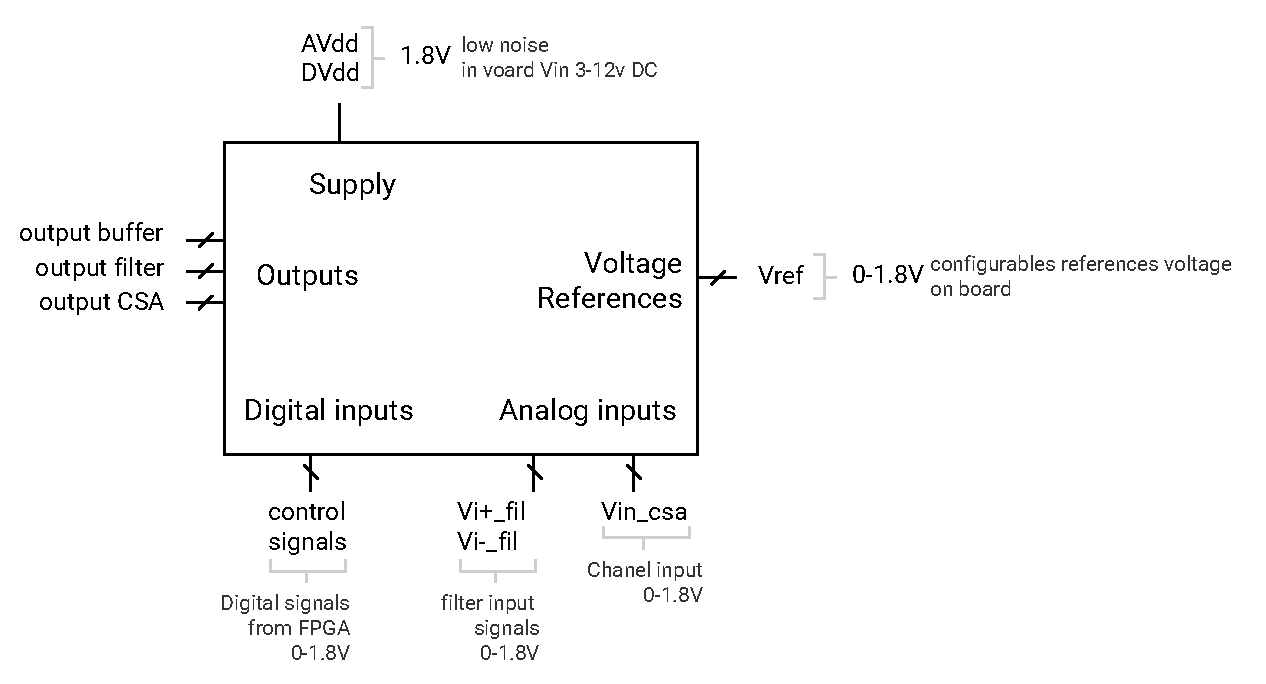
\includegraphics[width=6in]{./figures/especificiaciones-01}
	\caption{Diagrama general de los requisitos del IC.}\label{fig:thebean_spec}
\end{figure}



Para generar el control de las variables digitales, la plataforma de pruebas debe contar con una interfaz que permita comunicarse con un control digital. Otro de los aspectos importantes a considerar en los requisitos para la plataforma de pruebas, es la capacidad de operar \textit{on-line}, es decir, realizar continuas iteraciones de secuencias de entradas para distintas configuraciones y condiciones de operación del integrado, sin tener que re-programar el controlador. Esto implica contar con un protocolo que permita establecer una comunicación entre un computador y el controlador en tiempo real.

En resumen la plataforma de pruebas a implementar debe cumplir con los siguientes requisitos:
\begin{itemize}
\item Contar con reguladores de voltaje para generar la alimentación del IC the bean V2.
\item Poseer la capacidad de generar distintos voltajes para emular las entradas necesarias del sistema, lo cual debe implementarse en base a un conversor digital análogo (DAC) de 12 bits.
\item Debe contar con la capacidad de leer los datos de salida, para esto es necesario contar con dos conversores análogo digital (ADC) de 10 bits totalmente diferenciales.
\item Debe ser capaz de generar los voltajes de referencia para ajustar el punto de operación del integrado.
\item Implementar una interfaz que permita comunicarse directamente con un control digital.
\item Implementar junto al control un protocolo de comunicación, que permita el control \textit{on-line} del integrado.
\end{itemize}

 Dadas las especificaciones del problema, desarrollar un control basado en una FPGA aparece como la mejor opción. Debido a la versatilidad que ofrecen las FPGAs, es posible desarrollar un control tan específico como sea necesario. Además las FPGA comúnmente cuentan con un gran número de pines I/O lo cual permitiría controlar múltiples señales de control de forma paralela, aumentando la velocidad de procesamiento.	
 
 
Finalmente los objetivos específicos del trabajo presentado en esta tesis de pre-grado son:


\begin{enumerate}
\item Implementar una plataforma de pruebas que permita caracterizar bajo parámetros definidos un circuito integrado especifico llamado The bean V2.
\item Implementar dentro de la misma plataforma la capacidad de operar on-line.
\item Caracterizar el integrado dentro de las pruebas y parámetros establecidas bajo las consideraciones expuestas en este trabajo.
\end{enumerate}
\clearpage
\chapter{THE BEAN V2}
\label{chapter:theoretical}

El circuito integrado the bean V2 implementa un prototipo para la segunda iteración de the bean. En esta segunda iteración el principal objetivo es implementar un filtro que permita generar funciones de peso arbitrarias. 
Para llevar acabo este objetivo el integrado implementa el esquema mostrado en la figura \ref{introduccion:front-end-readout} por medio de dos bloques principales: un amplificador CSA y un filtro generador de formas de pulso, implementado por un integrador de condensadores conmutados de ganancia ajustable. La figura \ref{layout} muestra el \textit{layout} del integrado diseñado. En la sección \ref{appendix1} del Anexo se entrega una tabla con el detalle de la distribución de cada uno de  los pines del integrado.


	
%\begin{figure}[!h]
%	\centering
%	
%	\includegraphics[width=0.5\textwidth]{./figures/theorical/IC_layout}
%	\caption{\label{layout}The Bean V2 prototype layout.}
%\end{figure}

El esquema de la estructura general del circuito implementado por el IC se entrega en la figura \ref{thebean}. La primera etapa del IC consiste en un amplificador CSA, el cual se encarga de recibir la señal de entrada desde el detector y  generar un escalón de voltaje proporcional a la cantidad de carga inyectada. Junto con el amplificador, esta etapa cuenta con: un bloque destinado a generar la polarización del amplificador; un bloque para el control de la red de \textit{feedback}, que permite seleccionar la capacitancia de realimentación dependiendo del modo de operación; y por último, cuenta con un bloque de pre-carga para inyectar carga en la entrada con el objetivo de mover el \textit{baseline}\footnote{El baseline se define como el valor de la salida de un CSA cuando no se presenta estímulo en la entrada.} del CSA a un punto que optimice el rango de salida. En el IC también existe un segundo bloque CSA idéntico al anterior, con la diferencia de que posee la salida y la entrada conectadas, esto con el objetivo de poder generar y medir el \textit{baseline}.
	


%\begin{figure}[!t]
%	% XCircuit output "tx_ltspice.tex" for LaTeX input from tx_ltspice.eps
\def\putbox#1#2#3#4{\makebox[0in][l]{\makebox[#1][l]{}\raisebox{\baselineskip}[0in][0in]{\raisebox{#2}[0in][0in]{\scalebox{#3}{#4}}}}}
\def\rightbox#1{\makebox[0in][r]{#1}}
\def\centbox#1{\makebox[0in]{#1}}
\def\topbox#1{\raisebox{-0.60\baselineskip}[0in][0in]{#1}}
\def\midbox#1{\raisebox{-0.20\baselineskip}[0in][0in]{#1}}
\begin{center}
\scalebox{0.4}{
   \normalsize
   \parbox{17in}{
   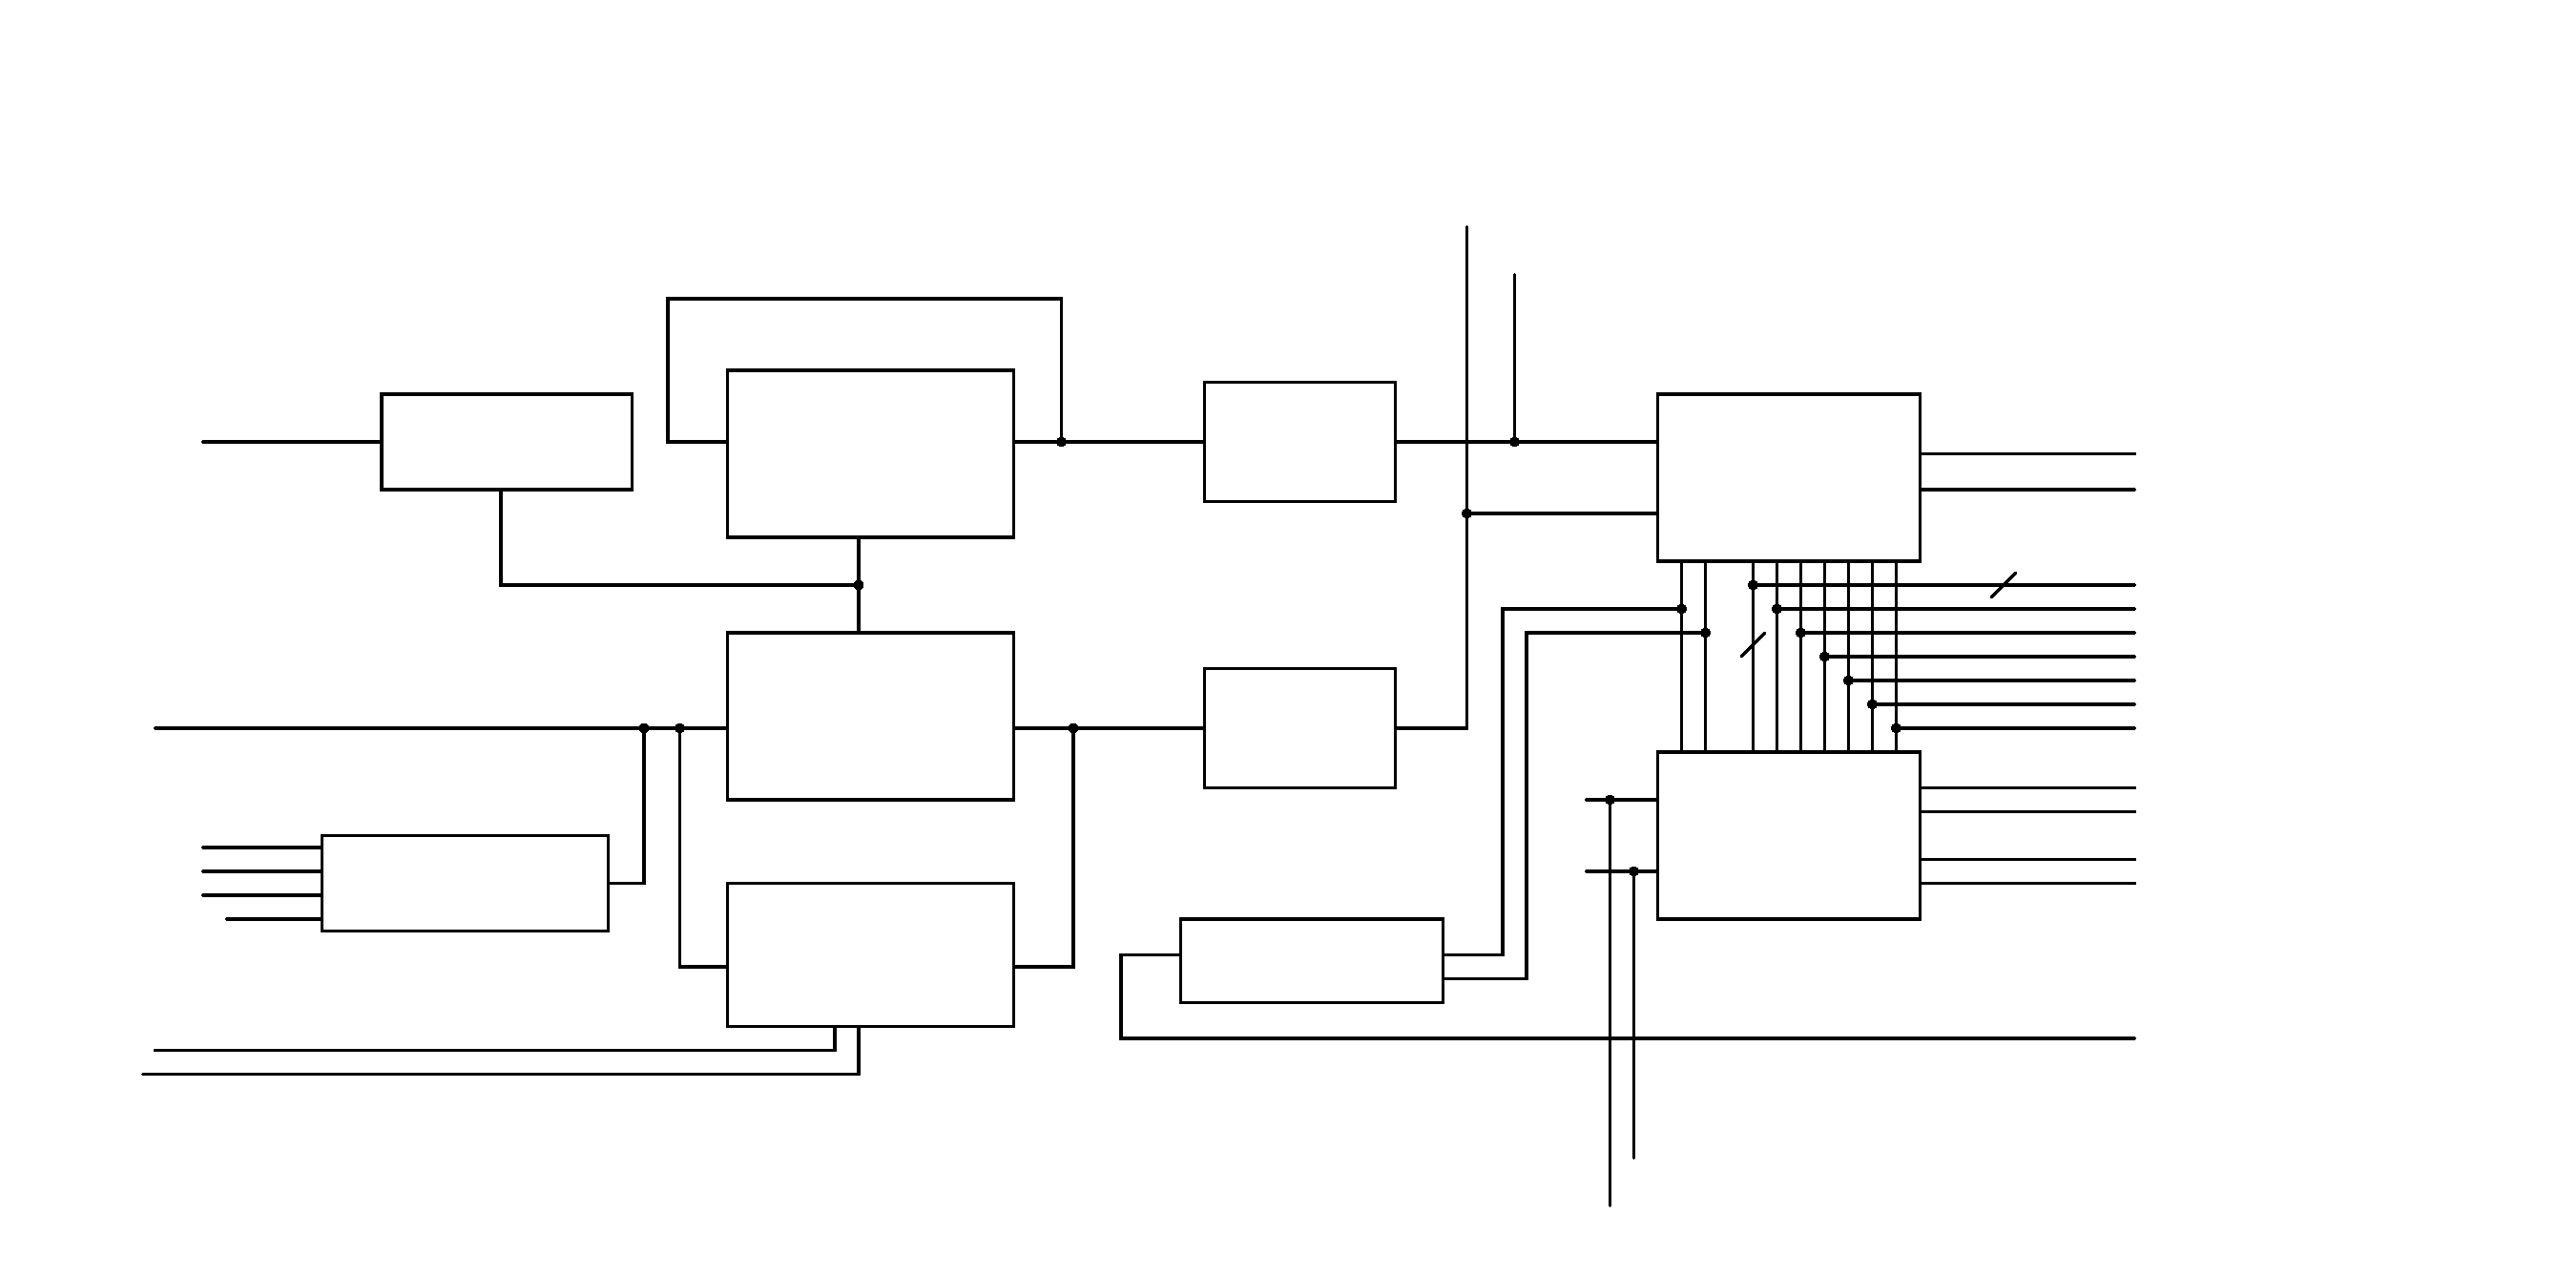
\includegraphics[scale=1]{./figures/theorical/thebeanv2.eps}\\
% translate x=1296 y=1280 scale 0.38
\putbox{0.06in}{5.72in}{1.2}{res\_bias\_ext}%
\putbox{0.06in}{3.72in}{1.2}{Vin\_csa}%
\putbox{0.06in}{2.89in}{1.2}{Vref\_prechar}%
\putbox{0.06in}{2.72in}{1.2}{clk\_prechar1}%
\putbox{0.06in}{2.56in}{1.2}{clk\_prechar2}%
\putbox{0.06in}{2.39in}{1.2}{C\_ext\_prechar}%
\putbox{0.06in}{1.47in}{1.2}{op\_mode}%
\putbox{0.06in}{1.31in}{1.2}{rst\_csa}%
\putbox{2.72in}{5.64in}{1.2}{CSA\_bias}%
\putbox{2.31in}{2.64in}{1.2}{pre\_charger}%
\putbox{5.31in}{2.22in}{1.2}{CSA\_ctrl}%
\putbox{5.31in}{1.89in}{1.2}{feedback}%
\putbox{5.56in}{5.56in}{1.2}{CSA}%
\putbox{5.56in}{3.72in}{1.2}{CSA}%
\putbox{8.56in}{5.64in}{1.2}{buffer}%
\putbox{8.56in}{3.64in}{1.2}{buffer}%
\putbox{8.31in}{2.06in}{1.2}{phase\_gen}%
\putbox{11.97in}{5.39in}{1.2}{Filter}%
\putbox{11.97in}{2.89in}{1.2}{Filter}%
\putbox{14.97in}{4.72in}{1.2}{CS\_Bx}%
\putbox{14.97in}{4.56in}{1.2}{out\_s}%
\putbox{14.97in}{4.39in}{1.2}{Vocm}%
\putbox{14.97in}{4.22in}{1.2}{hold}%
\putbox{14.97in}{4.06in}{1.2}{rst}%
\putbox{14.97in}{3.89in}{1.2}{sgn}%
\putbox{14.97in}{3.72in}{1.2}{Vicm}%
\putbox{14.97in}{5.64in}{1.2}{Vo+\_ch}%
\putbox{14.97in}{5.39in}{1.2}{Vo-\_ch}%
\putbox{14.97in}{3.31in}{1.2}{Vo-\_fil}%
\putbox{14.97in}{3.14in}{1.2}{Vo+\_fill}%
\putbox{14.97in}{2.81in}{1.2}{Vo-\_bp\_fill}%
\putbox{14.97in}{2.64in}{1.2}{Vo+\_bp\_fill}%
\putbox{14.97in}{1.56in}{1.2}{clk}%
\putbox{11.31in}{0.39in}{1.2}{Vin-\_fill}%
\putbox{11.14in}{0.06in}{1.2}{Vin+\_fill}%
\putbox{10.14in}{7.39in}{1.2}{Vout\_csa}%
\putbox{10.47in}{7.06in}{1.2}{baseline}%
   } % close 'parbox'
   } % close 'scalebox'
\end{center}

%	\caption{\label{thebean}The Bean V2 prototype layout.}
%\end{figure}

Ambas salidas tanto la del CSA como la del \textit{baseline} pasan por respectivos \textit{buffers}. Las salidas de ambos \textit{buffer} están disponibles para ser leídas en respectivos pines del integrado. Posteriormente ambas señales sirven de entrada para el filtro.

El filtro es implementado por un integrador totalmente diferencial de capacitores conmutados con capacitancia configurable por medio de señales digitales. Además cuenta con cuatro señales de control que permiten configurar el modo de operación controlando: el \textit{clock} de conmutación, el signo de la entrada del filtro, la procedencia de la señal de salida (la cual puede provenir desde la entrada o desde la salida del filtro), y la opción de poder mantener la señal a la salida con el fin de facilitar la lectura. Además el filtro necesita dos voltajes de referencia para fijar los valores de modo común tanto para la entrada como para la salida.
	Por último, existe una segunda versión del filtro para propósitos de pruebas y caracterización. Esta versión del filtro cuenta con las entradas conectadas directamente a pines del integrado, y comparte las señales de control y la polarización con el filtro antes mencionado.
	
 	
	

\section{Detalle del integrado}
 

\subsection{El CSA}

El objetivo de este bloque es convertir la carga generada por el detector en una señal de voltaje. La figura \ref{csa} muestra en detalle la forma en que es implementado dentro del IC. 

\begin{figure}[!h]
	\centering
	% XCircuit output "tx_ltspice.tex" for LaTeX input from tx_ltspice.eps
\def\putbox#1#2#3#4{\makebox[0in][l]{\makebox[#1][l]{}\raisebox{\baselineskip}[0in][0in]{\raisebox{#2}[0in][0in]{\scalebox{#3}{#4}}}}}
\def\rightbox#1{\makebox[0in][r]{#1}}
\def\centbox#1{\makebox[0in]{#1}}
\def\topbox#1{\raisebox{-0.60\baselineskip}[0in][0in]{#1}}
\def\midbox#1{\raisebox{-0.20\baselineskip}[0in][0in]{#1}}
\begin{center}
\scalebox{0.4}{
\normalsize
\parbox{9in}{
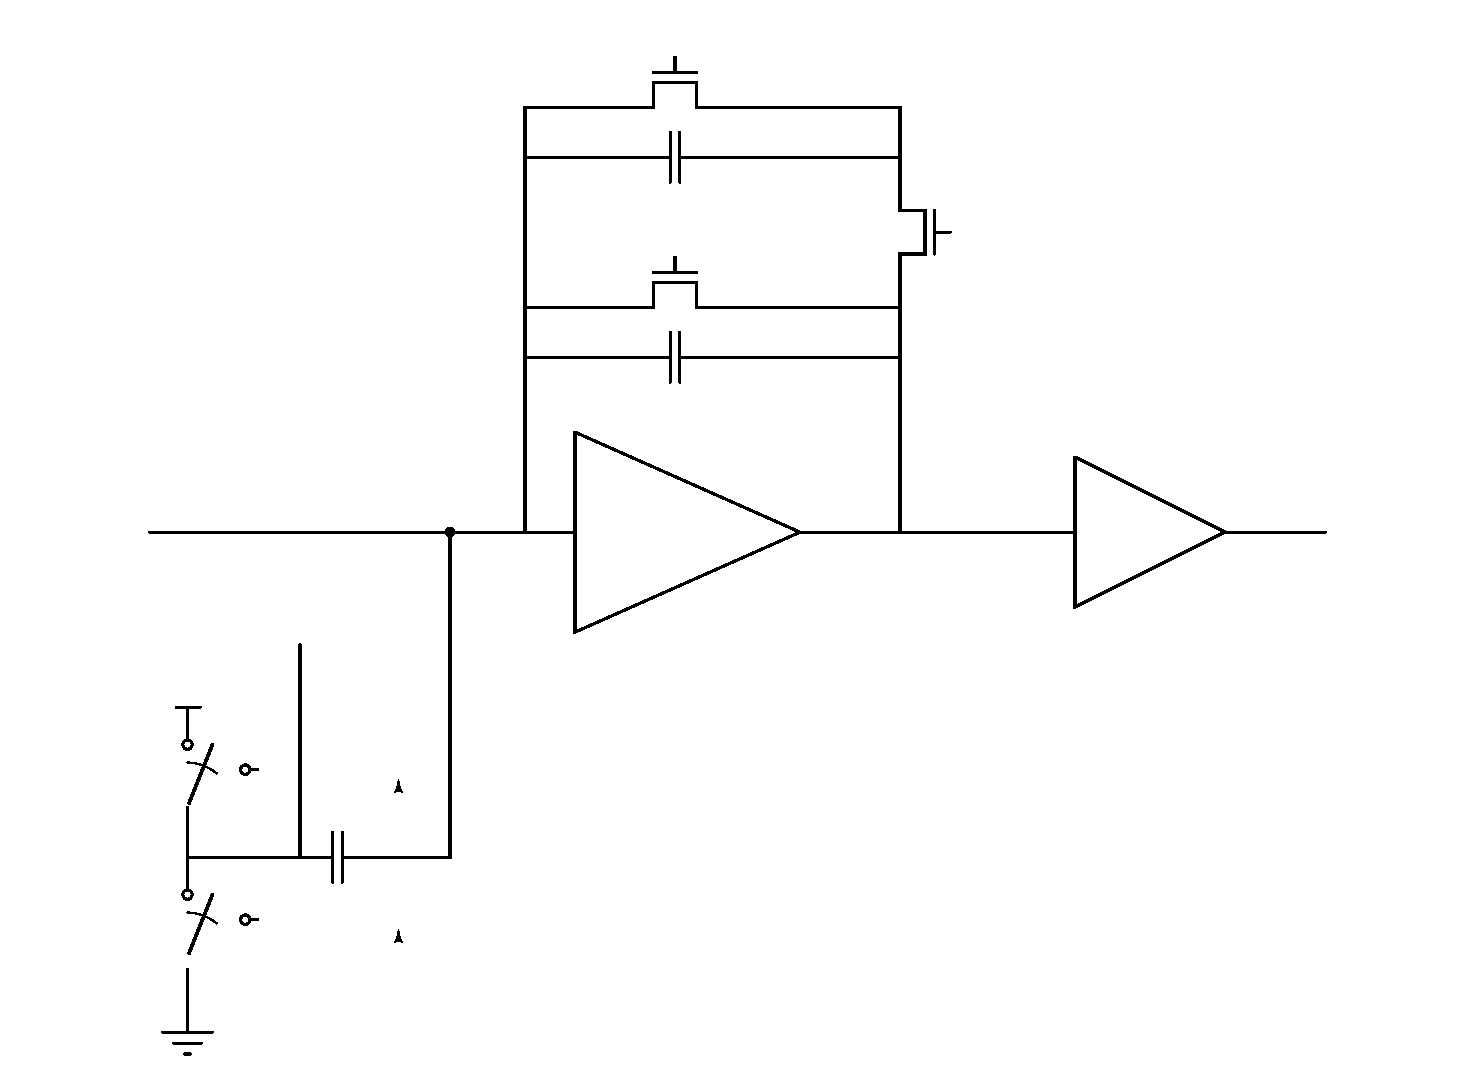
\includegraphics[scale=1]{./figures/theorical/csa_circuit2.eps}\\
% translate x=1152 y=860 scale 0.38
\putbox{0.22in}{3.62in}{1.2}{Vin\_csa}%
\putbox{0.72in}{2.45in}{1.2}{Vref\_pc}%
\putbox{1.56in}{2.87in}{1.2}{Cext\_pc}%
\putbox{4.06in}{5.54in}{1.2}{rst\_csa}%
\putbox{4.14in}{6.79in}{1.2}{rst\_csa}%
\putbox{6.39in}{5.54in}{1.2}{op\_mode}%
\putbox{8.72in}{3.62in}{1.2}{Vout\_csa}%
\putbox{0.14in}{1.87in}{1.2}{$\phi_1$\_pc}%
\putbox{0.06in}{1.04in}{1.2}{$\phi_2$\_pc}%
 } % close 'parbox'
 } % close 'scalebox'
\vspace{-\baselineskip} % this is not necessary, but looks better
\end{center}

	\caption{\label{csa}The Bean V2 prototype layout.}
\end{figure}

El CSA cuenta con dos condensadores de realimentación los cuales permiten configurar el valor de la capacitancia de realimentación $C_F$, por medio de la señal digital \verb+op_mode+. Así $C_F= C_{Cal}$ en el modo DCal y $C_F= C_{Cal}+ C_{Op}$ en el modo SDT. De este modo, es posible implementar distintas ganancias para los diferentes modos de operación. Por otro lado, la señal \verb+rst_csa+ permite implementar la función de \textit{reset} en la red de realimentación descargando la carga almacenada en los condensadores.

 Debido a la configuración con la cual fue implementado el CSA, el baseline se establecerá aproximadamente a $V_T$ o $0.5V$, sin embargo, la región de operación de alta ganancia se encuentra aproximadamente a los $0.4V$ de los rieles. Para solucionar este problema es que el CSA cuenta con circuito de pre-carga, el cual inyecta una cantidad conocida de carga para mover el baseline más cerca de los $0.4V$.
 

\subsection{Pre-charger}


El circuito de pre-carga fue diseñado para inyectar carga a la entrada del CSA con el objetivo de ajustar el baseline y a la vez para cumplir con propósitos de calibración.
 En la imagen \ref{Cir_vin} se muestra una versión simplificada del circuito. Esta formado por dos switches implementados con transistores y un condensador $C_{PC}$ el cual esta conectado a la entrada del CSA. Para cambiar el valor de la capacitancia de este condensador (modo SDT) existe la posibilidad de conectar un condensador externo en paralelo por medio de la señal \verb+cap_prechar_ext+.
 
 
La forma en que se controla el circuito de pr-ecarga se basa en dos señales de clock desfasadas no sobrepuestas. Cuando la primera señal esta activa ($\phi_1$), el extremo izquierdo del condensador queda conectado a un voltaje de referencia externo $V_{DD\_ref}$ configurable por medio de la señal \verb+V_ref_prechar+. Posteriormente, cuando la segunda señal esta activa ($\phi_2$), el extremo izquierdo es conectada a tierra. En cada transición de $\phi_2$ a $\phi_1$ el condensador inyecta una carga de $Q_{CP}=C_{CP} \cdot V_{DD\_ref}$ en la entrada del CSA. Esto provoca una variación de voltaje en la salida de $\Delta V =-C_{CP} \cdot V_{DD\_ref}/C_F$, en donde $C_F$ es la capacitancia de realimentación. La inyección de carga se realiza justo después de que el CSA es habilitado, reduciendo el voltaje de baseline a la salida. 

\begin{figure}
\def\putbox#1#2#3{\makebox[0in][l]{\makebox[#1][l]{}\raisebox{\baselineskip}[0in][0in]{\raisebox{#2}[0in][0in]{#3}}}}
\def\rightbox#1{\makebox[0in][r]{#1}}
\def\centbox#1{\makebox[0in]{#1}}
\def\topbox#1{\raisebox{-\baselineskip}[0in][0in]{#1}}
\def\midbox#1{\raisebox{-0.5\baselineskip}[0in][0in]{#1}}
\begin{flushleft}
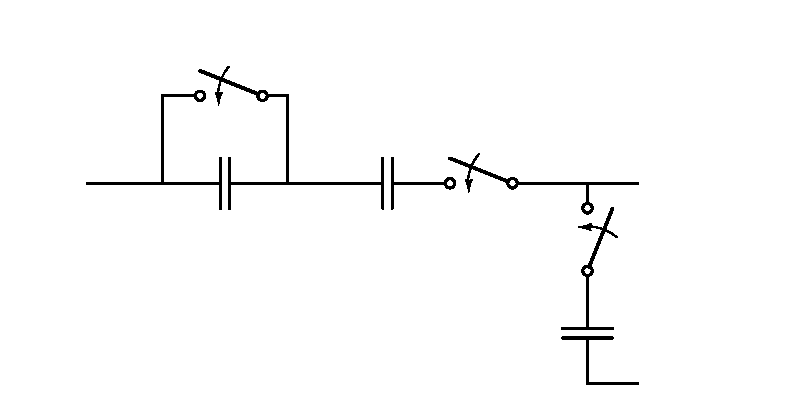
\includegraphics[width=1\textwidth]{./figures/theorical/Injector_de_carga.eps}\\
% translate x=816 y=166 scale 0.38
\putbox{0.06in}{1.42in}{Vin}%
\putbox{1.22in}{2.34in}{JP9}%
\putbox{1.22in}{1.00in}{C36}%
\putbox{1.22in}{0.75in}{0.5pF}%
\putbox{2.31in}{1.00in}{C37}%
\putbox{2.31in}{0.75in}{27pF}%
\putbox{2.81in}{1.75in}{JP10}%
\putbox{4.22in}{1.42in}{Vin\_csa}%
\putbox{4.22in}{0.09in}{Cext\_pc}%
\putbox{3.14in}{0.50in}{C38}%
\putbox{3.14in}{0.25in}{25pF}%
\putbox{3.22in}{1.00in}{JP11}%
\end{flushleft}
\caption{\label{Cir_vin}Circuito de inyección de carga en la tarjeta, para simular un detector.}
\end{figure}

\subsection{Filtro}
La segunda gran etapa del integrado corresponde a un filtro, el cual posee la ventaja de poder implementar funciones de peso arbitrarias, permitiendo de este modo, generar filtros que maximicen la SNR ayudando a reducir el ruido del proceso de lectura tal como se describe en Avila er al 2013. Este filtro es un prototipo para the Bean V2.

Con el objetivo de generar funciones de peso arbitrarias, el filtro implementa la ecuación \ref{theorical:ecuacion_f_z}, por medio de un integrador de capacitores conmutados totalmente diferencial. El esquema general de este circuito se puede apreciar en la figura \ref{theorical:filtro}.

El filtro posee dos fases de operación. Durante la primera fase, $\phi_1$, ocurre el muestreo,  la diferencia de voltaje de la entrada  carga ambos capacitores $C_S$. Durante la segunda fase, $\phi_2$, el cortocircuito virtual de la entrada del OTA fuerza a que la carga almacenada en $C_S$ sea transferida hacia el capacitor $C_F$. De este modo, el voltaje en la salida al final de la segunda fase es igual al voltaje en la iteración anterior más $C_S \Delta V_i^k / C_F$. De este modo la ganancia del filtro es proporcional a la razón entre las capacitores $C_S$ y $C_F$.
 
La capacitancia $C_S$ es implementada por un conjunto de capacitores en paralelo que pueden conectarse por medio de switches. De este modo, es posible cambiar digitalmente el valor de la capacitancia $C_S$. Esto último permite implementar una ganancia configurable digitalmente. Las señales \verb+CSB0+ a \verb+CSB5+ realizan el control digital de los respectivos capacitores.

El filtro también cuenta con un grupo de señales que permiten configurar su operación. El multiplexor de entrada permite intercambiar las señales de entrada, permitiendo controlar el sentido de la integración, lo cual es utilizado para implementar las pendientes negativas de las funciones de peso\footnote{Denominado CDS}. El multiplexor de salida, por otro lado, permite evitar el filtro en caso de que se estime necesario para STD mode o para modos de calibración. También cuenta con una señal de \textit{reset} que permite desaguar la carga de los capacitores $C_S$ y $C_F$. Posee una señal para mantener la salida en estado de \textit{hold} con propósito de facilitar mediciones. 

El OTA cuenta con una red interna de control de modo común de salida(CMFB). Tanto los voltajes de modo común de entrada como el de salida quedan quedan disponibles para ser ajustados por referencias externas. 
 



\begin{equation}
F(z)= \sum_{j=0}^{N-1} a_{N-j}z^{-1}
\label{theorical:ecuacion_f_z}
\end{equation}

\begin{figure}[!h]
	\centering
	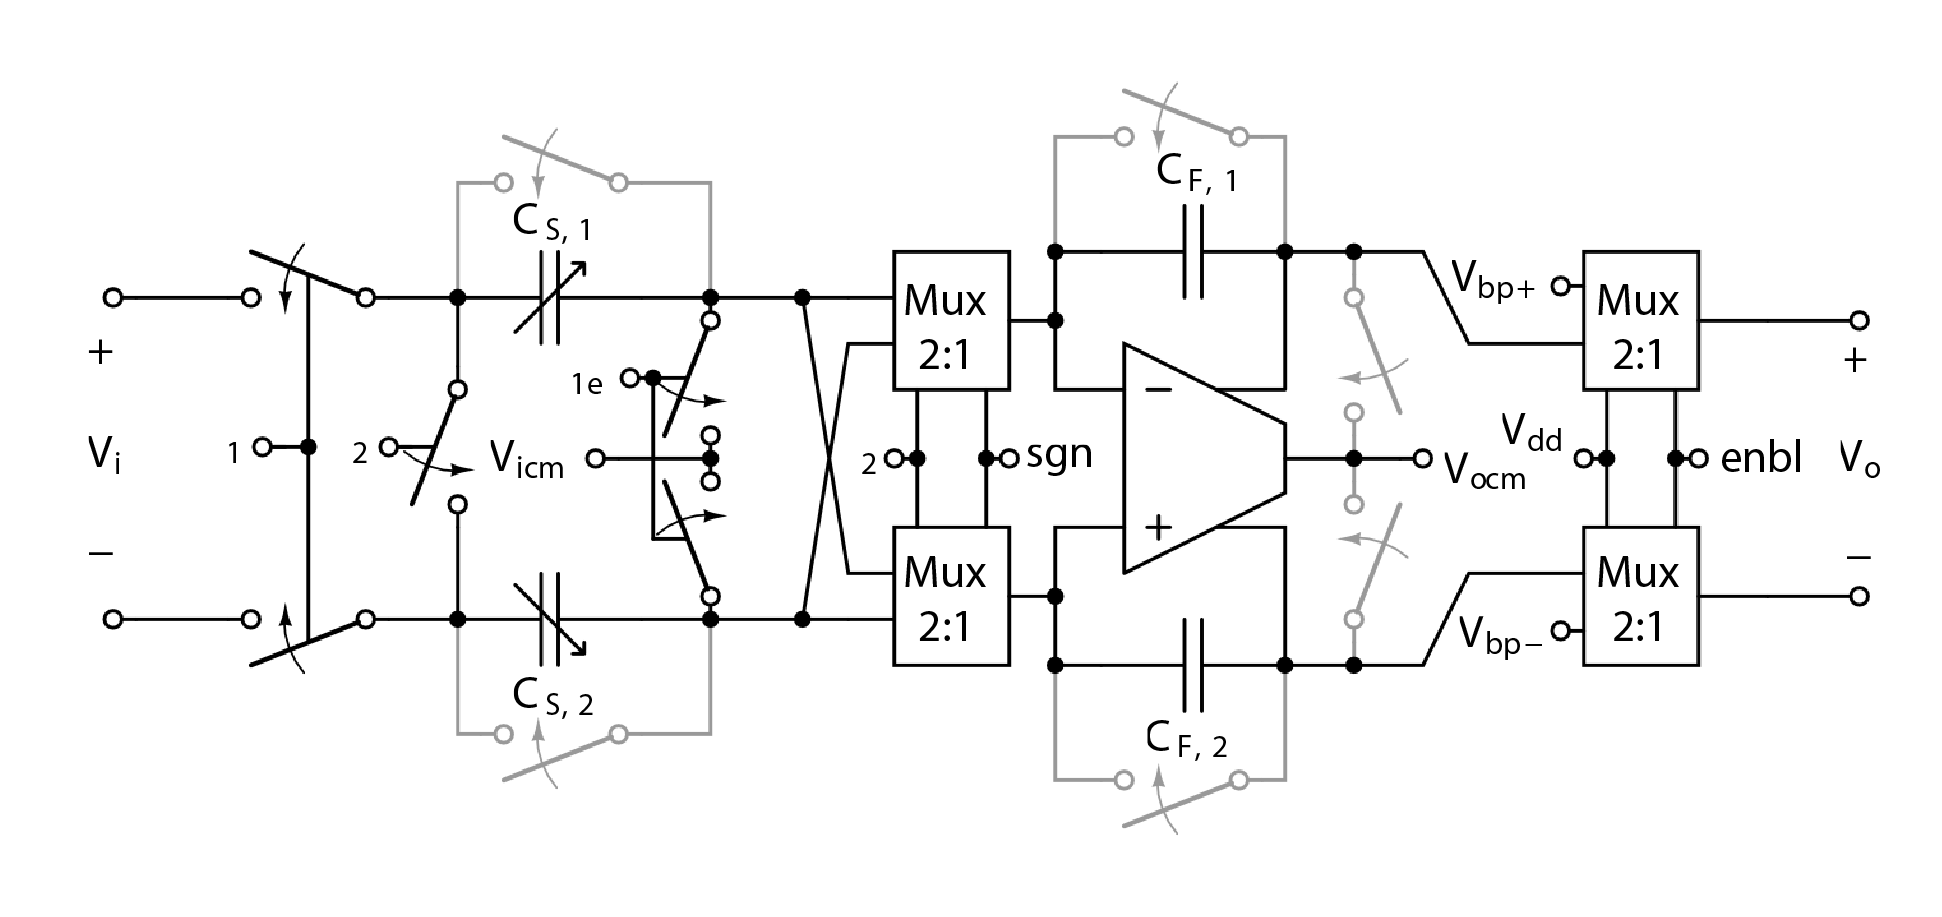
\includegraphics[width=1\textwidth]{./figures/theorical/filtro.png}
	\caption{\label{theorical:filtro}The Bean V2 prototype layout.}
\end{figure}

\section{Pruebas y diagramas de tiempo}





\subsection{Diagramas de tiempo}
\begin{figure}[!t]
	\centering
	\includegraphics[width=5in]{./figures/theorical/test_filter_after_omni.eps}
	\caption{Filter functionality simulation. $V_\textit{in}=0.1\,V$ and $\text{gain}=0.25\,V/V$.}\label{fig:test_filter_after_omni}
\end{figure}

\begin{figure}[!t]
	\centering
	\includegraphics[width=4.4in]{./figures/theorical/gain_curves.pdf}
	\caption[Filter step response for constant input for the 64 possible programmable gains.]{Filter step response for constant input for the 64 possible programmable gains. \mbox{$V_\textit{in}=0.1\,V$} and \mbox{$T_s=40\,\text{ns}$}.}\label{fig:gain_curves}
\end{figure}

\begin{figure}[!t]
	\centering
	\includegraphics[width=3.6in]{./figures/theorical/sim_wf}
	\caption{SPICE-simulated weighting function. $\tau=8\,\text{ns}$, $N=16$ and $T_s=19.25\,\text{ns}$.}\label{fig:sim_wf}
\end{figure}

\subsection{Diseño de pruebas}

\begin{figure}[!t]
	\centering
	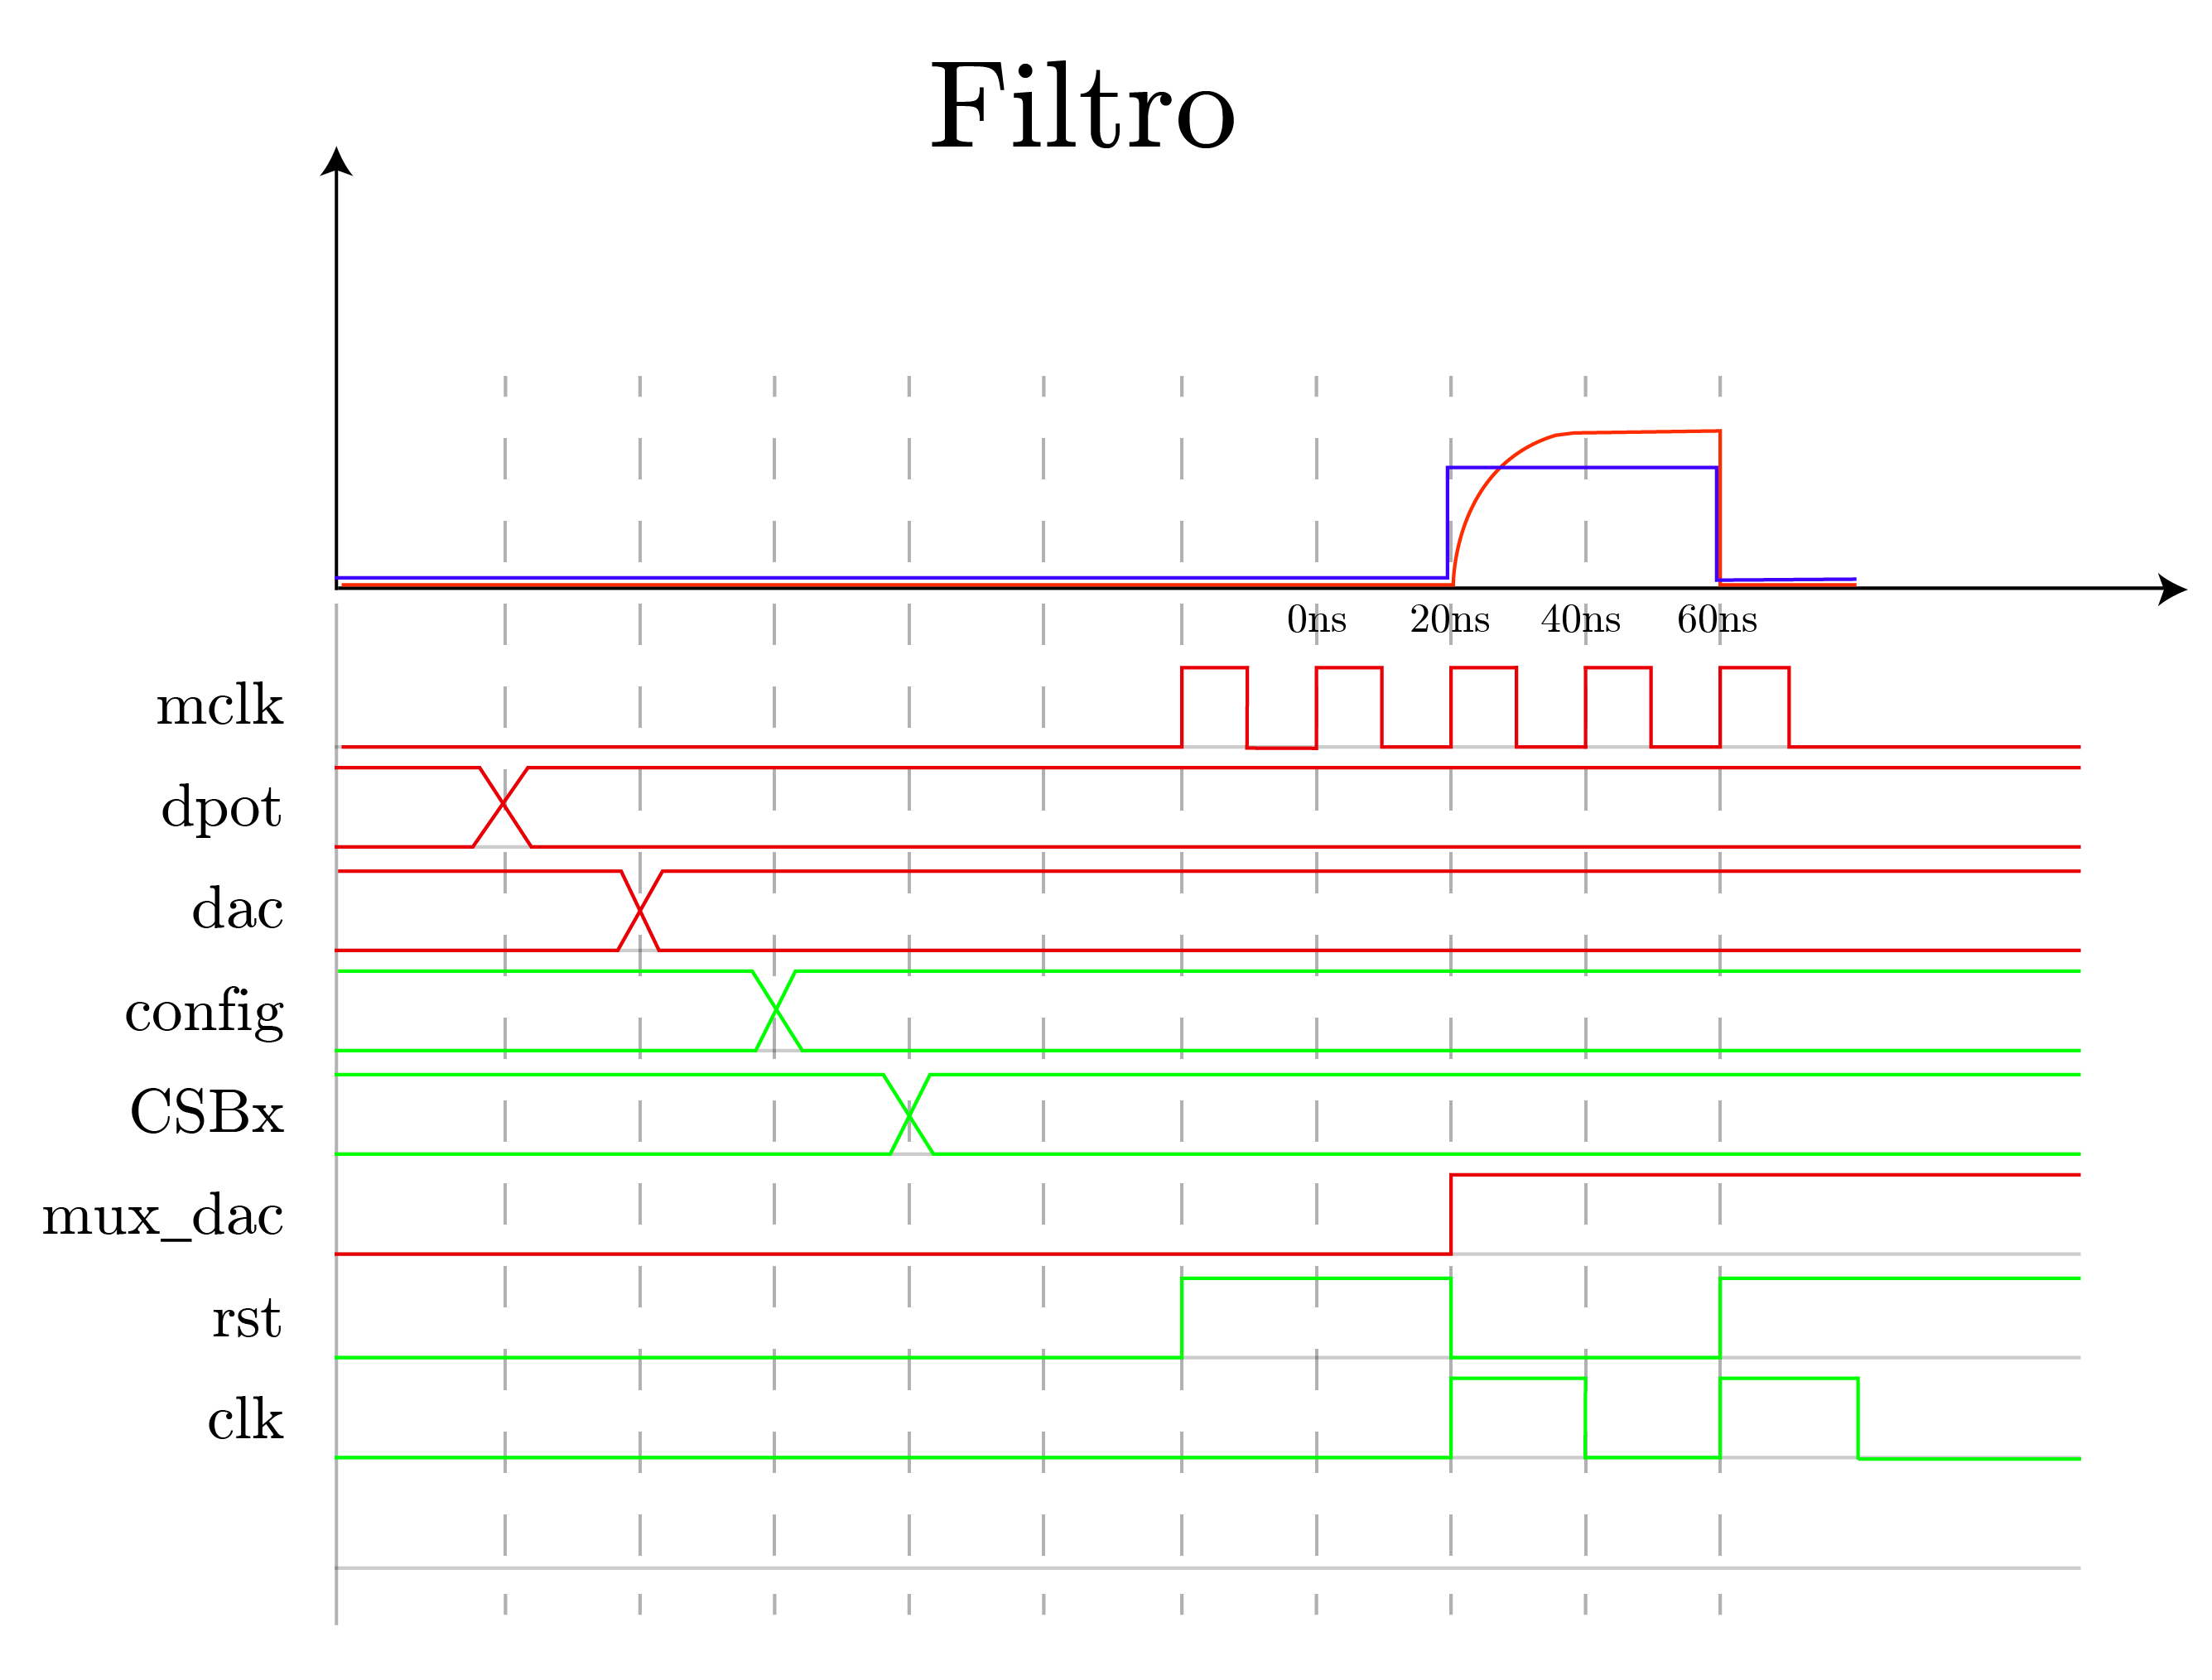
\includegraphics[width=1\textwidth]{./figures/theorical/tiempos_filtro.png}
	\caption{Diagrama de señales para las pruebas realizadas al filtro .}\label{fig:diagramafiltro}
\end{figure}

\begin{figure}[!t]
	\centering
	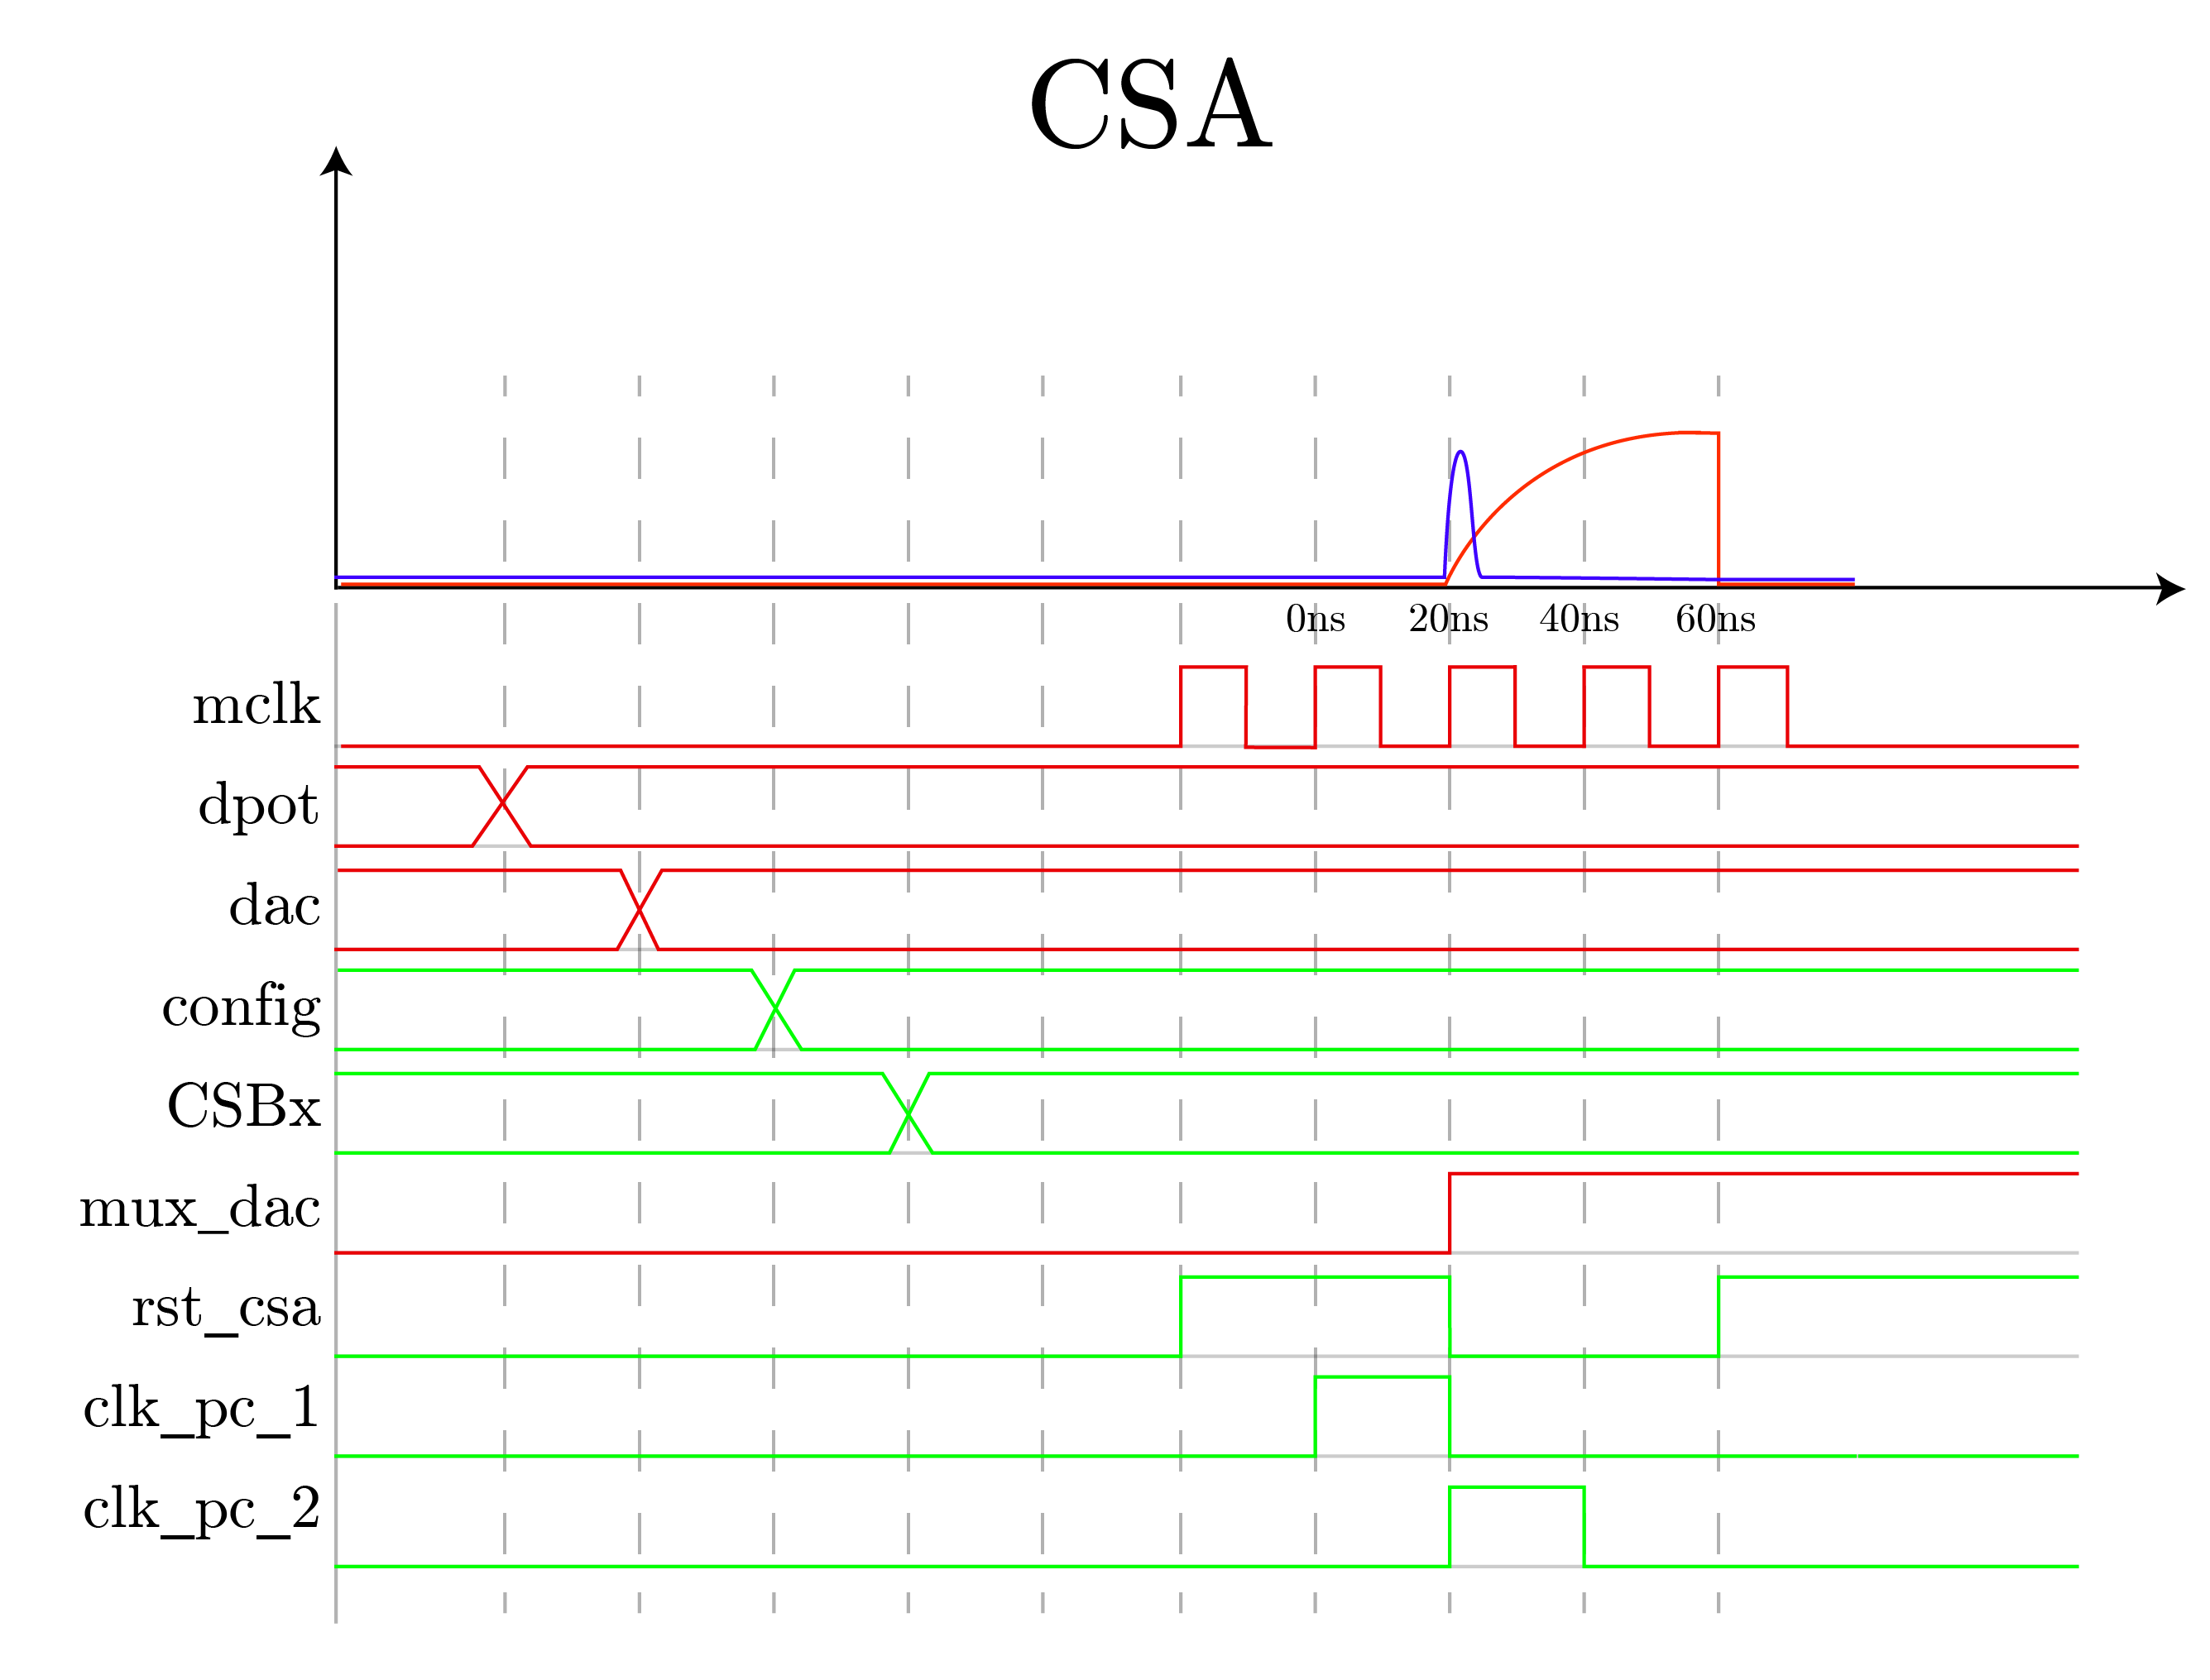
\includegraphics[width=1\textwidth]{./figures/theorical/tiempos_csa.png}
	\caption{Diagrama de señales para las pruebas realizadas al CSA.}\label{fig:diagramacsa}
\end{figure}




\clearpage
\chapter{A SC FILTER FOR ARBITRARY WEIGHTING FUNCTION SYNTHESIS}
\label{chapter:filter}
\hyphenation{topology simplicity}
\section{Introduction}

%In particle physics experiments, where the results from the collisions are inferred from the measurement of electric charge in various sets of detectors \citep{gatti101,radeka101}, noise sets a fundamental limit for the charge measurement resolution \citep{degeronimo102}. In such experiments, the typical detector \mbox{front-end} circuit comprises a \mbox{charge-sensitive} amplifier (CSA) and a filter, often referred to as pulse shaper. The former is used to convert the input charge signal, coming from the detector electrodes, into a voltage signal, and is responsible for most of the noise present in the readout circuit signal path \citep{degeronimo101,degeronimo102}. The filter is used to convert the voltage signal at the CSA output into a shaped voltage pulse, in order to maximize the \mbox{signal-to-noise} ratio (SNR) at the measurement time.  

%A current trend on particle physics instrumentation is to implement this filter in the discrete time domain, which allows to synthesize weighting functions (WFs) with virtually any shape, producing near-optimum filters. In \citep{diego101} a novel mathematical framework for a design-oriented analysis of discrete-time filters was presented. One of the greatest benefits of this framework is that it allows to easily compute the optimal discrete-time filter that maximize the SNR in a typical detector front-end circuit, a difficult task to achieve using the traditional methods intended for continuous-time networks. In this work, a generic filter designed to be flexible enough to synthesize arbitrary weighting functions is presented, 

One of the greatest benefits of the mathematical framework presented in \citep{avila101} is that it allows to easily find the optimal discrete-time filter that minimizes the noise of a typical detector front-end circuit, a difficult task to undertake using the traditional methods for continuous-time networks. The filter presented in this chapter is designed to be flexible enough to synthesize arbitrary weighting functions with an adequate resolution. Therefore, it could be used to synthesize the optimal filter described above. The filter is a prototype of the front-end filter for the Bean V2, which was introduced in Chapter~\ref{chapter:problem}. Hence, the main specifications are derived from the Bean specifications. Also, power, noise and size budgets of the referred IC are taken as constraints.

There are two common options for implementing the required filter. The simplest is to digitize the CSA output directly with a fast analog-to-digital converter (ADC)  - $N$ times faster than the typical used ADC, with $N$ the number of desired samples - and then process the samples in the digital domain, whereas the other option is to use a custom \mbox{switched-capacitor} (SC) network as a filter, without changing the ADC requirements. Considering the Bean timing constraints, the former option is not feasible, given that such fast ADC would exceed the available power and size budgets. Hence, the SC solution was finally chosen.


\section{System-Level Design}
As mentioned in the previous Chapter, to synthesize arbitrary weighting functions the front-end filter should be designed to have a  discrete-time transfer function $F(z)$ given by
\begin{equation}
F(z) = \sum_{j=0}^{N-1}a_{N-j} \hspace{0.1em}z^{-j} \label{eq:filter_tf}
\end{equation}
where $a_i$ are the filter gain coefficients and $N$ is the filter length. Fig.~\ref{fig:filter_post} shows a simplified circuit diagram of a fully-differential SC integrator designed to implement $F(z)$. Some control logic and switches have been purposely omitted.

The filter has two phases of operation. During the sampling phase, $\phi_1$, the input voltage charges  both $C_S$ capacitors. During the amplification phase, $\phi_2$, the OTA input virtual short circuit forces charge from capacitors $C_S$ to be transferred to capacitors $C_F$. Thus, at the end of $\phi_2$, the filter output voltage is equal to its value in the previous cycle, plus $C_S V_i/C_F$. Also, an early version of $\phi_1$, $\phi_{1e}$, is used in the sampling phase to implement Bottom-Plate Sampling \citep{haigh101}, a technique used to reduce the charge injection from switches.

In this configuration, the filter instantaneous gain is given by the ratio of the capacitors $C_S$ and $C_F$.  Considering that in order to obtain arbitrary coefficients the filter gain must be programmable, either $C_S$ or $C_F$ should be implemented with a variable capacitor. For simplicity, capacitor $C_S$ was selected for this purpose. The OTA input multiplexers are used to swap the OTA inputs, and therefore, to invert the sign of the filter gain. The OTA output common-mode level is set by the OTA's internal common-mode feedback (CMFB) circuit, whereas the input common-mode level is set by the external reference $V_\textit{icm}$. The OTA output multiplexers are used to bypass the filter for the SDT operation mode and for diagnostic purposes.


\begin{figure}[!t]
	\centering
	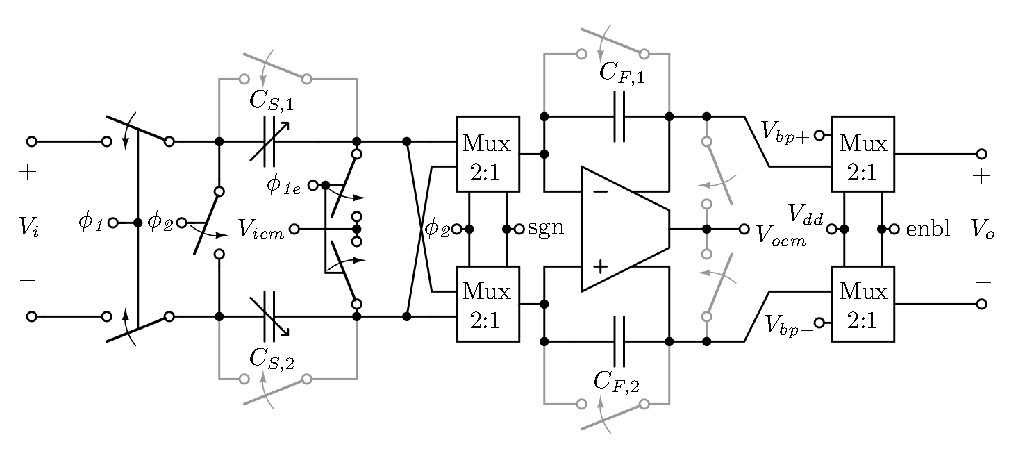
\includegraphics[width=6in]{./Figures/Filter/filter_post.eps}
	\caption{Simplified filter schematic. Reset switches are depicted in gray.}\label{fig:filter_post}
\end{figure}

\subsection{Filter Specifications}

Table \ref{tab:filter_specs} summarizes the filter specifications derived from the Bean specifications (Table \ref{tab:bean_specs}). Also, the CSA output specifications and the ADC input specifications were taken into account. The sampling frequency is $51.95\,\text{MHz}$. Thus, each integration subcycle is $19.25\,\text{ns}$ long. Since each subcycle involves two phases, sampling and holding, each phase has only $9.625\,\text{ns}$ for settling. Considering this time, to assure a dynamic error of $0.1\,\%$ (to meet the dynamic range specification) the amplifier must have a \mbox{worst-case} \mbox{closed-loop} bandwidth of $f_u = 118\,\text{MHz}$ (without considering slew-rate regime). Also, a static error of $0.1\,\%$ is required, which implies an OTA open-loop gain of at least $60\,\text{dB}$. 

\begin{table}[!t]
	\begin{center}
		\begin{tabular}{|l|l|}\hline
			{\bf Specification} & {\bf Value} \\ \hline\hline
			Modes of operation & SDT and DCal \\ \hline
			Input swing & 0.9 V or close \\ \hline
			Output swing & 1 V or close \\ \hline
			Dynamic range & 10 bits \\ \hline
			Gain resolution & 6 bits (7.8 mV/V - 0.5 V/V) \\ \hline
			Noise budget & $1.25\times Q_n^2$ \\ \hline
			Operation speed & $51.95\,\text{MHz}$ \\ \hline
			Power consumption & Minimize\\\hline
		\end{tabular}
		\vspace*{5pt}
		\caption{Filter specifications summary, where $Q_n^2$ is the readout ADC quantization noise.}\label{tab:filter_specs}
	\end{center}
\end{table}

%Besides the specifications required to implement arbitrary weighting functions, 

%
%In a SC integrator the noise should be analyzed at the two clock phases and then by added
%
%After $N$ integration cycles and assuming an arbitrary $C_S$ at each cycle, the contribution from noise sampled at $\phi_1$ can be computed as
%\begin{equation}
%\overline{V_{\phi_1}^2} = 2 kT \sum_{i=1}^{N} \frac{1}{C_{F_i}}\left(1 + \frac{C_S}{C_{F_i}}\right)
%\end{equation}
%
%In a proper design, switches resistance will be much smaller than $1/\beta g_\textit{m,eff}$, so noise contribution at $\phi_2$ can be assumed dominated by OTA noise. In a one stage OTA
%
%\begin{equation}
%\overline{V_{\phi_2}^2} = \frac{2 N_f kT}{g_\textit{meff}} \sum_{i=1}^{N} \frac{1}{\beta_i C_{Ltot_i}}
%\end{equation}
%
%where $N_f$ is a noise factor dependent on the OTA topology, for a recycling folded cascode
%
%\begin{equation}
%N_f \approx \left(1+\frac{g_{mf}}{g_{meff}}+\frac{g_{ml}}{g_{meff}}\right)
%\end{equation}
%
%
%In a two stage miller compensate OTA the noise is given by (citar a alumno de tom lee, calculo de ruido termico):
%\begin{equation}
%\overline{V_{\textit{filteramp}}^2}\approx 2N\left\{\frac{\gamma}{\beta}\cdot \frac{kT}{C_C}\left(1+\frac{g_{mxx}}{g_{mx}}\right)+\frac{kT}{C_{\textit{Ltot}}}\left[1+\gamma\left(1+\frac{g_{myy}}{g_{my}}\right)\right]\right\}\label{eq:noise_miller_ota}
%\end{equation}
%Where $C_C$ upper bounded by the amplifier speed requirement, looking at the unitary frequency 
%\begin{equation}
%f_u \approx \beta \frac{g_{min}}{2\pi C_C}
%\end{equation}
%
%With $\beta=1$ (worst case scenario), $g_\text{min}$ around a few $mS$ (which is given for a typical OTA solution only considering the gain and frequency requeriments) and considering the restriction for $f_u$, $C_C$ should be around a few hundred of $\textit{fF}$, which replaced in Eq.~\ref{eq:noise_millter_ota} won't complain the noise requirements for the OTA, so a one stage solution should be used.
%
%To obtain enough gain in one stage a folded cascade amplifier is a suitable candidate, using (citar paper de analysis orientado al diseno de ruido), the noise given by a folded cascade ota can be approximated by
%
%\begin{equation}
%\overline{v_{\textit{in}}^2} = \frac{4 \gamma kT}{g_{{min}}} \left(1+y\right)
%\end{equation}
%
%where $y \approx \nicefrac{g_{{mf}}}{g_\text{min}}+\nicefrac{g_{{ml}}}{g_{min}}$, since $g_{mI}$ is larger compared to $1/r_{oL}$ and $1/(r_{oI}\parallel r_{oF})$ the noise contributions of $M_{CF}$ and $M_{CL}$ can be neglected


\section{Circuit Design}
\subsection{Operational Transconductance Amplifier}
The previous version of the Bean uses a two-stage Miller-compensated OTA as the filter amplifier. However, this topology does not lead to a feasible design given the filter specifications, mainly, because of the existing trade-off between noise and bandwidth, resulting from the Miller capacitor. For this version of the Bean, a \mbox{single-stage} OTA topology was chosen, as it can theoretically meet the filter specifications.  A folded cascode (FC) OTA would be the first candidate to implement this amplifier, because of its good balance between gain, speed, input-output swing and complexity. Nonetheless, the settling-time specification would require high bias currents due to the slew-rate limitation, which would come into conflict with the power budget. The recycling folded cascode OTA (RFC) \citep{assaad101}, a small variation over the FC OTA, was chosen to overcome this limitation, since it exhibits an enhanced transconductance, gain, and slew-rate (SR) over the conventional FC OTA for the same power and size budgets.

In a traditional FC OTA, folding transistors conduct most of the current and generally have the largest transconductance. However, their role is only limited to providing a folding node for the small signal current \citep{assaad101}. In a RFC OTA (Fig.~\ref{fig:OTA_post}), a small modification over the conventional FC topology allows to use the folding transistors as additional drivers for the small signal input. Therefore, they are used to enhance the effective transconductance of the amplifier. Also, this modification entails additional enhancements over the conventional FC OTA, such as higher and symmetrical SR, higher output resistance and higher \mbox{crossover-frequency}.

In a voltage-controlled voltage source (VCVS), such as the filter amplifier, the low-frequency \mbox{open-loop} gain can be calculated as $|A_V| = G_\textit{m,eff}  \cdot R_\textit{o}$, where $G_\textit{m,eff}$ is the effective transconductance, defined as the ratio of the incremental short-circuit output current to the input voltage, and $R_o$ is the output resistance, defined as the resistance seen at the amplifier output when no input is applied \citep{rashid101}. In a RFC OTA the effective transconductance can be approximated to:
\begin{equation}
G_\textit{m,eff} \approx g_\textit{m,in}(1+K)\label{eq:gmeff}
\end{equation}
where $K$ is the current mirror ratio between transistors $M_f$ and $M_\textit{aux,3}$. Also, the output resistance can be approximated to:
\begin{equation}
R_\textit{o} \approx g_\textit{m,cf}r_\textit{o,cf}\left(\left(r_\textit{o,in}\parallel r_\textit{o,aux3} \right) \parallel \left(g_\textit{m,cl} r_\textit{o,cl} r_\textit{o,l}\right)\right)
\end{equation}

Considering that the RFC OTA is a single-stage amplifier, and assuming a proper design, the dynamic behavior of the open-loop filter will be dominated by the output node resistance and the load capacitance, $C_L$, so other time constants can be ignored. For a RFC OTA, the unity-gain bandwidth, $\omega_u$, is given by:
\begin{equation}
\omega_u = \frac{G_\textit{m,eff}}{C_L}
\end{equation}
Once integrated in the filter, all non-dominant poles and zeros will be beyond the \mbox{unity-gain} frequency. Thus, the closed-loop bandwidth, $\omega_c$, can be approximated to:
\begin{equation}
\omega_c = \beta \frac{G_\textit{m,eff}}{C_\textit{L,tot}}
\end{equation}
where $\beta$ is the feedback factor, given by
\begin{equation}
\beta \approx \frac{C_F}{C_F+C_S+C_\text{parasitic}}
\end{equation}
and $C_\textit{L,tot}$ is the total load capacitance, given by:
\begin{equation}
C_\textit{L,tot} = C_L + (1-\beta)C_F
\end{equation}
where $C_\text{parasitic}$ is the parasitic capacitance at the OTA input node.

In a RFC OTA the SR is symmetrical and enhanced $K$ times over the FC OTA for the same power consumption. Considering $I_\textit{tail}$ as the bias current of the transistor $M_\textit{tail}$, the SR can be computed as:
\begin{equation}
\text{SR} = \frac{2 K I_\textit{tail}}{C_L}
\end{equation}

In a SC integrator, noise is sampled at both clock phases, namely $\phi_1$ and $\phi_2$. Thus, to calculate the filter output-referred total integrated noise, both noise contributions must be calculated separately and added up in quadrature. After $N$ integration cycles and assuming an arbitrary $C_S$ at each cycle, the contribution from noise sampled at $\phi_1$ can be computed as:
\begin{equation}
\overline{V_{\phi_1}^2} = 2 kT \sum_{i=1}^{N} \frac{1}{C_F}\left(1 + \frac{C_{S_i}}{C_F}\right)
\end{equation}
In a proper design, switch resistances will be much smaller than $1/(\beta g_\textit{m,eff})$, so noise at $\phi_2$ can be assumed to be dominated by the OTA noise \citep{vleugels101}. Thus, the noise contribution at $\phi_2$ can be approximated to:
\begin{equation}
\overline{V_{\phi_2}^2} \approx \frac{2 N_f kT\gamma}{g_\textit{m,eff}} \sum_{i=1}^{N} \frac{1}{\beta_i C_{Ltot_i}}
\end{equation}
where $N_f$ is a noise factor dependent on the single-stage OTA topology, for a RFC:
\begin{equation}
N_f \approx \frac1{1+K}\left(\frac{1+K^2}{1+K} + \frac{g_\textit{m,f}}{g_\textit{m,in}} + \frac1{1+K}\frac{g_\textit{m,l}}{g_\textit{m,in}}\right) \label{eq:Nf}
\end{equation}
Table~\ref{tab:OTA_sizes} shows the parameter values for the OTA design. Transistor sizes were calculated using equations \ref{eq:gmeff} to \ref{eq:Nf} and a semi-exhaustive search script, with tabulated pre-simulated data and using the $g_m/I_D$ design technique \citep{silveira101}. Computational power was not a problem at this point. However, for a deeper optimal design, a bigger domain must be chosen (not increasing the boundaries but increasing the domain resolution) and an intelligent algorithm must be used, e.g like the use of Support Vector Machines in \citep{bernardinis101} to reduce the feasible domain of solutions.  SPICE simulations predict an \mbox{open-loop} DC gain of $72\,\text{dB}$, a crossover frequency of $150\,\text{MHz}$, and a phase margin of $75^\circ$ measured with an $0.4\,\text{pF}$ load.


\begin{figure}[!t]
	\centering
	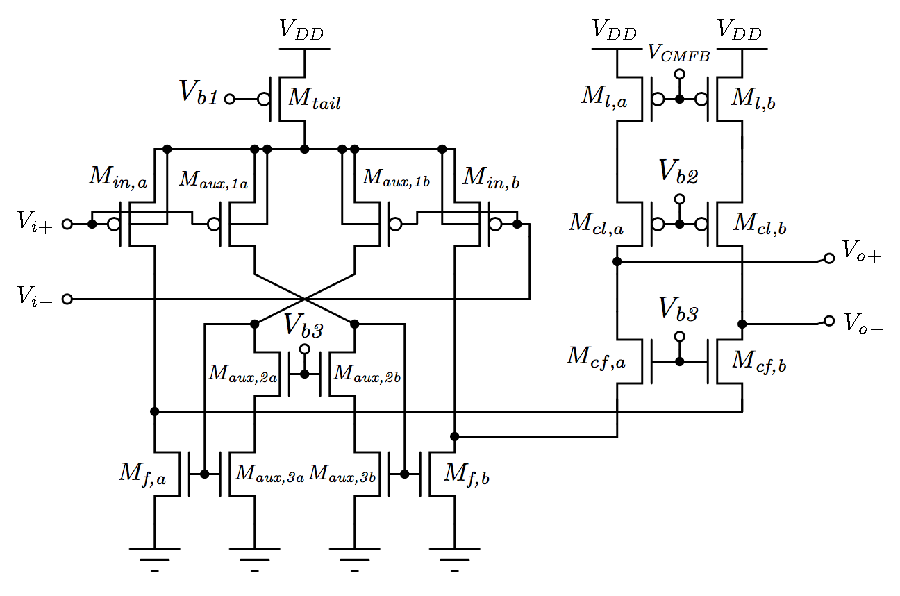
\includegraphics[width=5.5in]{./Figures/Filter/OTA_post.eps}
	\caption[Recycling folded cascode OTA schematic.]{Recycling folded cascode OTA schematic. Three terminal NMOS and PMOS devices are with their bodies tied to ground and $V_\textit{DD}$ respectively. CMFB circuit is shown in Fig.~\ref{fig:CMFB_post}}\label{fig:OTA_post}
\end{figure}
\begin{figure}[!t]
	\centering
	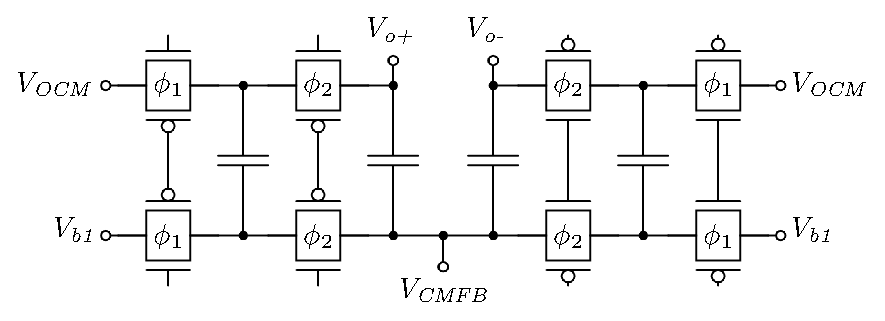
\includegraphics[width=4.6in]{./Figures/Filter/CMFB_post.eps}
	\caption{OTA discrete-time commmon-mode feedback circuit schematic.}\label{fig:CMFB_post}
\end{figure}
\begin{figure}[!t]
	\centering
	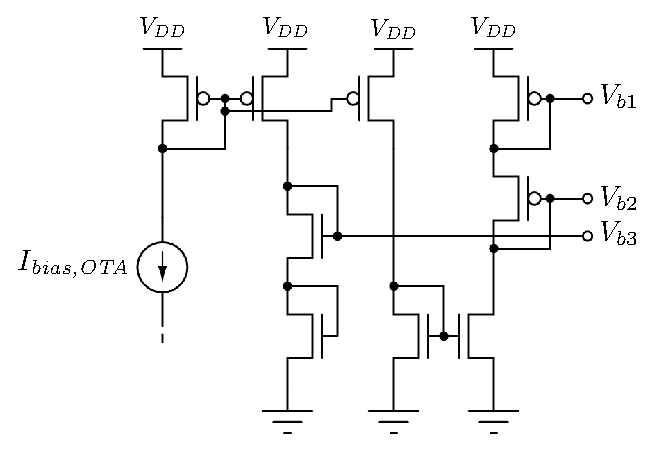
\includegraphics[width=4in]{./Figures/Filter/bias_ota_post.eps}
	\caption{OTA bias network schematic.}\label{fig:bias_ota_post}
\end{figure}
\begin{table}[!t]
	\begin{center}
		\begin{tabular}{|l|r|r|r|r|}\hline
			Transistor & Bias current & $g_m/I_D$ & $W$ & $L$ \\ \hline\hline
			$M_\text{in}$ & $51.3\,\mu\text{A}$  & $14.9\,\text{mS}/\text{mA}$  & $48\,\mu\text{m}$ & $0.36\,\mu\text{m}$ \\ \hline
			$M_\text{tail}$ & $201.7\,\mu\text{A}$  & $8.2\,\text{mS}/\text{mA}$  & $64\,\mu\text{m}$ & $0.45\,\mu\text{m}$ \\ \hline 
			$M_\text{f}$ & $100.6\,\mu\text{A}$  & $8.7\,\text{mS}/\text{mA}$  & $8\,\mu\text{m}$ & $0.45\,\mu\text{m}$ \\ \hline
			$M_\text{cf}$ & $49.3\,\mu\text{A}$  & $11.7\,\text{mS}/\text{mA}$  & $8\,\mu\text{m}$ & $0.45\,\mu\text{m}$ \\ \hline
			$M_\text{cl}$ & $49.3\,\mu\text{A}$  & $10.7\,\text{mS}/\text{mA}$  & $16\,\mu\text{m}$ & $0.3\,\mu\text{m}$ \\ \hline
			$M_\text{l}$ & $49.3\,\mu\text{A}$  & $7.6\,\text{mS}/\text{mA}$  & $32\,\mu\text{m}$ & $1\,\mu\text{m}$ \\ \hline
			$M_\text{aux,1}$ & $49.6\,\mu\text{A}$  & $15\,\text{mS}/\text{mA}$  & $48\,\mu\text{m}$ & $0.36\,\mu\text{m}$ \\ \hline
			$M_\text{aux,2}$ & $49.6\,\mu\text{A}$  & $9.5\,\text{mS}/\text{mA}$  & $2\,\mu\text{m}$ & $0.18\,\mu\text{m}$ \\ \hline
			$M_\text{aux,3}$ & $49.6\,\mu\text{A}$  & $6\,\text{mS}/\text{mA}$  & $4\,\mu\text{m}$ & $0.45\,\mu\text{m}$ \\ \hline
		\end{tabular}
		\vspace*{5pt}
		\caption{Filter OTA design values.}
		\label{tab:OTA_sizes}
	\end{center}
\end{table}

\subsection{Variable Capacitor}
Fig.~\ref{fig:cap_array_post} shows the schematic of the binary-weighted array used to implement the variable capacitor $C_S$. All capacitors $C_{S,bn}$ were designed as a parallel connection of unity metal-insulator-metal (MIM) capacitors $C_u=8.1\,\text{fF}$  (with an area of $2.7\,\micro\text{m}\times2.7\,\micro\text{m}$), which for matching purposes were also used to implement capacitor $C_F$. CMOS switches were sized to meet filter speed specifications.  Switch control signals will be directly bonded out off-chip. A \mbox{serial-programmable} memory to store the filter coefficients, and which will be connected directly to these control signals - to avoid the \mbox{unnecessary} use of IC pads -, will be included in future revisions of the Bean.

\begin{figure}[!t]
	\centering
	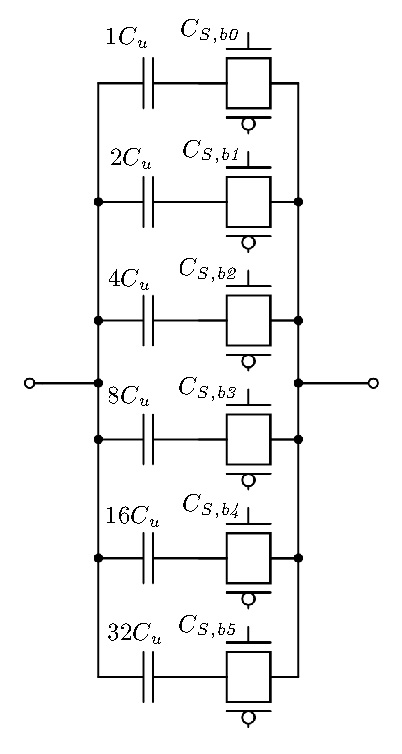
\includegraphics[width=1.8in]{./Figures/Filter/cap_array_post.eps}
	\caption{6-bit programmable capacitor.}\label{fig:cap_array_post}
\end{figure}

\subsection{Rail-to-Rail buffer}
A signal buffer is required to buffer some of the Bean prototype voltages for scope probing. The buffer must be able to drive a $8\,\text{pF}$ load at a reasonable speed and power dissipation, with truly rail-to-rail input and output voltages. Fig.~\ref{fig:buffer_post} shows the schematic of a rail-to-rail operational amplifier (op-amp) used to implement a unity-gain voltage buffer amplifier.

The two-stage op-amp consists of a rail-to-rail constant-$g_m$ input stage \citep{hogervorst101}, composed by two complementary input pairs and an electronic zener diode, $M_\text{in1}$-$M_\text{in2}$, $M_\text{ip,a}$-$M_\text{ip,b}$ and $M_\textit{zp}$-$M_\textit{zn}$,  followed by folded-cascode, current-mirroring loads, \mbox{$M_\textit{cln1}$-$M_\textit{ln1}$}, $M_\textit{cln2}$-$M_\textit{ln2}$, $M_\textit{clp1}$-$M_\textit{lp1}$ and $M_\textit{clp2}$-$M_\textit{lp2}$, and a class-AB output \citep{hogervorst102}, $M_\textit{op}$-$M_\textit{on}$. Transistors $M_\textit{sn1}$-$M_\textit{sn2}$ and $M_\textit{sp1}$-$M_\textit{sp2}$ implement a translinear loop \citep{analogessentials}, producing the voltage shifts necessary to set the output devices quiescent current consumption.

As in most of two-stage amplifiers, stability must be assured with a proper compensation scheme. In this design, capacitor $C_C$, also known as Miller capacitor, is placed to lower the frequency of the dominant pole and to increase the frequency of the secondary pole, and thus, it helps to increase the phase margin of the amplifier, while resistor $R_Z$ is used to shift to infinity the right-half plane zero that appears because adding $C_C$. Since $C_C$ is calculated as a function of the input stage's total transconductance, the constant-$g_m$ compensation technique used for the input stage helps to maintain a constant frequency response over all the input common mode range.

To assure predictable bias currents and a true rail-to-rail input and output voltage ranges, a proper bias network must be designed. Fig.~\ref{fig:bias_buffer_post} shows the schematic of the bias network used for this op-amp \citep{baker101}. All bias voltages are driven by cascoded current mirrors, which have high output resistance in order to reduce the effect of $V_{ds}$ over the mirrored current. Transistor sizes were calculated to assure a maximum amplifier output swing and mirror currents were chosen to maintain a good tradeoff between mirrored currents sensibility and bias network power consumption. 

Table~\ref{tab:buffer_sizes} shows the parameter values for the rail-to-rail buffer design. Transistor sizes were calculated with the same methodology as that used for the OTA design. SPICE simulations predict an open-loop DC gain of $103$\,dB, a crossover frequency of $52$,MHz, and a phase margin of $72\,^\circ$ measured with an $8\,\text{pF}$ load. 
\begin{table}[!t]
	\begin{center}
		\begin{tabular}{|l|r|r|r|r|}\hline
			Transistor & Bias current & $g_m/I_D$ & $W$ & $L$ \\ \hline\hline
			$M_\textit{in}$ & $10.4\,\mu\text{A}$ & $21.2\,\text{mS}/\text{mA}$ & $12.8\,\mu\text{m}$ & $0.45\,\mu\text{m}$ \\ \hline
			$M_\textit{ip}$ & $9.2\,\mu\text{A}$ & $19.4\,\text{mS}/\text{mA}$ & $40\,\mu\text{m}$ & $0.45\,\mu\text{m}$ \\ \hline
			$M_\textit{tp}$ & $60.6\,\mu\text{A}$ & $7.4\,\text{mS}/\text{mA}$ & $20\,\mu\text{m}$ & $0.45\,\mu\text{m}$ \\ \hline
			$M_\textit{tn}$ & $62.9\,\mu\text{A}$ & $9.2\,\text{mS}/\text{mA}$ & $6.4\,\mu\text{m}$ & $0.45\,\mu\text{m}$ \\ \hline
			$M_\textit{lp}$ & $26.3\,\mu\text{A}$ & $9.1\,\text{mS}/\text{mA}$ & $10\,\mu\text{m}$ & $0.45\,\mu\text{m}$ \\ \hline
			$M_\textit{clp}$ & $16\,\mu\text{A}$ & $14.2\,\text{mS}/\text{mA}$ & $20\,\mu\text{m}$ & $0.45\,\mu\text{m}$ \\ \hline
			$M_\textit{ln}$ & $25.2\,\mu\text{A}$ & $10.9\,\text{mS}/\text{mA}$ & $3.2\,\mu\text{m}$ & $0.45\,\mu\text{m}$ \\ \hline
			$M_\textit{cln}$ & $16\,\mu\text{A}$ & $16.8\,\text{mS}/\text{mA}$ & $6.4\,\mu\text{m}$ & $0.45\,\mu\text{m}$ \\ \hline
			$M_\textit{op}$ & $282\,\mu\text{A}$ & $9\,\text{mS}/\text{mA}$ & $100\,\mu\text{m}$ & $0.45\,\mu\text{m}$ \\ \hline
			$M_\textit{on}$ & $282\,\mu\text{A}$ & $10.7\,\text{mS}/\text{mA}$ & $32\,\mu\text{m}$ & $0.45\,\mu\text{m}$ \\\hline
		\end{tabular}
		\vspace*{5pt}
		\caption{Rail-to-rail buffer main design values.}
		\label{tab:buffer_sizes}
	\end{center}
\end{table}
\begin{figure}[!t]
	\centering
	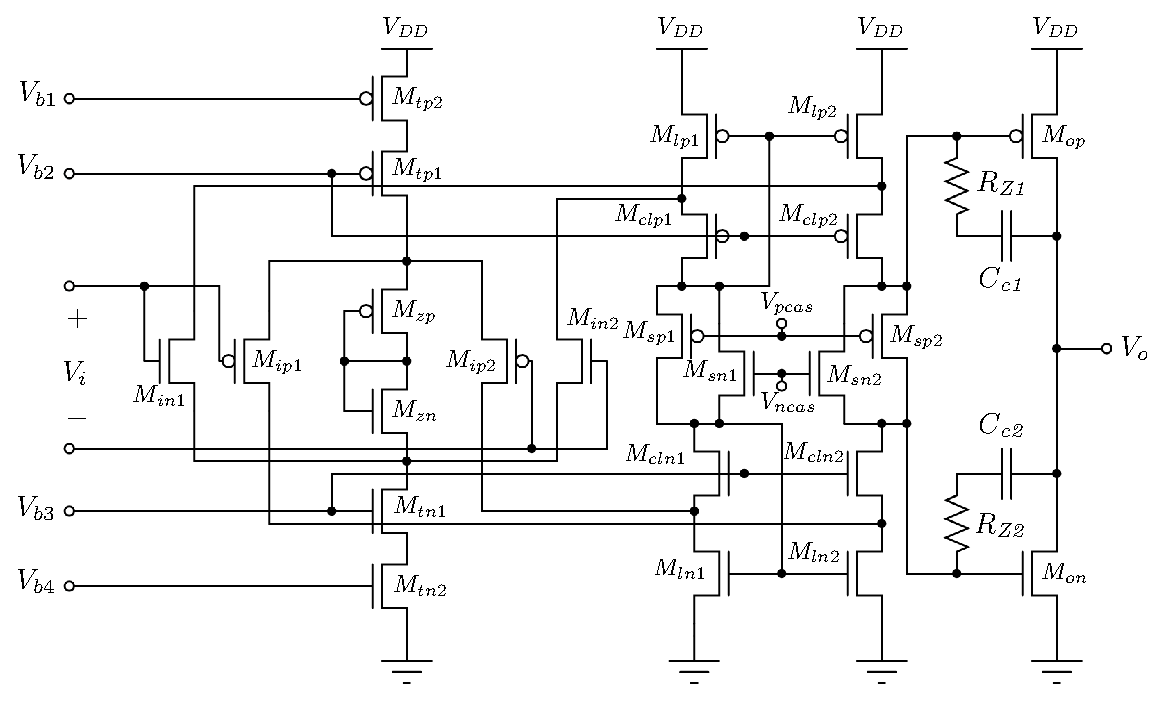
\includegraphics[width=6in]{./Figures/Filter/buffer_post.eps}
	\caption{Rail-to-rail operational amplifier schematic.}\label{fig:buffer_post}
\end{figure}
\begin{figure}[!t]
	\centering
	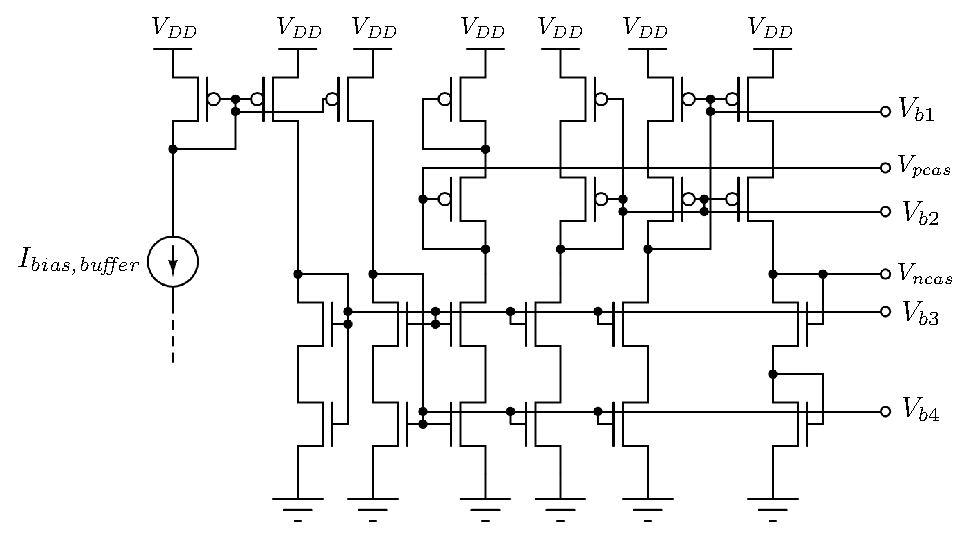
\includegraphics[width=5in]{./Figures/Filter/bias_buffer_post.eps}
	\caption{Op-amp bias network schematic.}\label{fig:bias_buffer_post}
\end{figure}


\subsection{IC bias network}
The previous version of the Bean uses a voltage distribution scheme to bias all the circuits in the IC, but it can cause big problems due to IR drop and process gradients, so a more common current distribution scheme was chosen for this iteration of the design \citep{murmann101}.  The main disadvantage of this architecture is the additional current consumption, but this drawback is marginal compared to the entire IC power budget and the obtained benefits. To achieve a good power supply rejection (PSR), a supply-insensitive bias network was chosen to implement the global bias cell, from which all the bias currents are generated. Fig.~\ref{fig:bias_all_post} shows a diagram of the current distribution bias scheme. For simplicity, only three current branches are illustrated, although five were used in the final design. Fig.~\ref{fig:bias_filter_post} shows the schematic of a $\beta$-multiplier bias circuit, the architecture selected to implement the supply-insensitive bias network. This consist of a \mbox{self-biased} \mbox{current-reference} network, a \mbox{start-up} circuit, because there are two possible operating points, and a cascode current mirror. The $\beta$-multiplier is an example of a circuit that uses positive feedback. The addition of the resistor kills the closed loop gain\footnote{A positive feedback system can be stable if its closed loop gain is less than one.}. However, if the parasitic capacitance of this resistor is large, it will increase the loop gain and push the feedback system closer to instability. If the resistor, for example, is bonded out off-chip to set the current, it is likely that this bias circuit will oscillate \citep{baker101}.

\begin{figure}[!t]
	\centering
	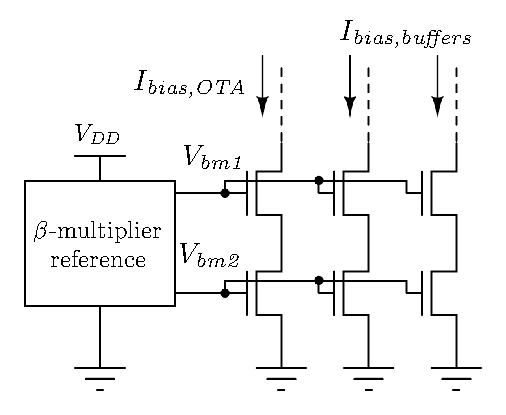
\includegraphics[width=3in]{./Figures/Filter/bias_all_post.eps}
	\caption{Current distribution bias scheme.}\label{fig:bias_all_post}
\end{figure}
\begin{figure}[!t]
	\centering
	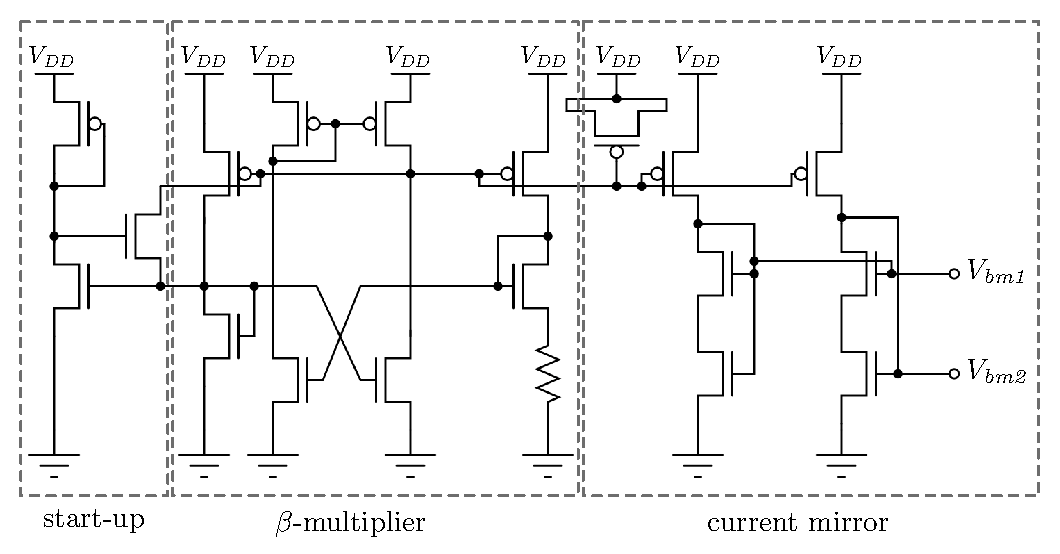
\includegraphics[width=6in]{./Figures/Filter/bias_filter_post}
	\caption{$\beta$-multiplier bias schematic.}\label{fig:bias_filter_post}
\end{figure}
\clearpage
\chapter{RESULTS}
\label{chapter:results}

\section{The Bean V2 prototype Implementation}
The Bean V2 prototype was designed for a standard mixed-signal $180\text{-nm}$ \textsc{cmos} process. This iteration of the Bean includes two standalone structures: a trimmed version a readout channel, which includes two CSA (one with its input and output connected, to generate the baseline voltage\footnote{The baseline is defined as the CSA DC output voltage after reset, when no input has been applied.}), a pre-charger circuit, the designed SC filter and output buffers; and an isolated version of the filter with its inputs directly bonded out off-chip.  Both structures will be tested separately, thus control signals and reference voltages for both filters are tied together. Also, a logic circuit to generate the non-overlapping two-phase clock was included. Future revisions of the prototype will include a 10-bit SAR ADC and a digital memory within the channel.

Fig.~\ref{fig:IC_layout} shows the layout of the Bean V2 prototype; for a detailed description of the IC pinout, see Appendix~A. Each channel cell was designed to have a pitch lower than $190\,\mu\text{m}$. If the number of channels is increased to the nominal value of $32$, the IC will be approximately $6\,\text{mm}$ tall, which can be fit into four mini@sic sub-blocks according to the Europractice rules. After including the ADC and the digital memory, channel length is expected to be lower than $1\,\text{mm}$.

\begin{figure}[!t]
	\centering
	\includegraphics[width=5in]{./Figures/IC_layout}
	\caption{The Bean V2 prototype layout.}\label{fig:IC_layout}
\end{figure}

The SC filter, shown in Fig.~\ref{fig:filter_layout}, has a total area of $185\,\mu\text{m}\times 332\,\mu\text{m}$, and was laid out to resemble the components spatial distribution of the circuit in Fig.~\ref{fig:filter_post}. The filters outputs, the main CSA output and the baseline voltage are buffered out off-chip using the rail-to-rail amplifiers (connected as unity-gain buffers) shown in Fig.~\ref{fig:buffer_layout}. The CSA and the filter OTA are depicted in Figs.~\ref{fig:csa_layout} and \ref{fig:ota_layout} respectively. All structures were carefully side-shielded with multiple guard-rings. Also, to mitigate the effects of cross-chip gradients,  the \mbox{common-centroid} technique and dummy devices were used in the layout of the filter OTA and the rail-to-rail op-amps. These considerations were not taken into account for the CSA layout, since mismatch is not critical for this cell because of the size of its transistors and because it is a single-ended device. As mentioned in the previous chapter, capacitors $C_F$ and $C_S$ were implemented with a parallel connection of unity MIM capacitors. To prevent copper-dishing effects, both capacitors were surrounded by dummy capacitors implemented with the same unity capacitors.

\begin{figure}[!t]
	\centering
	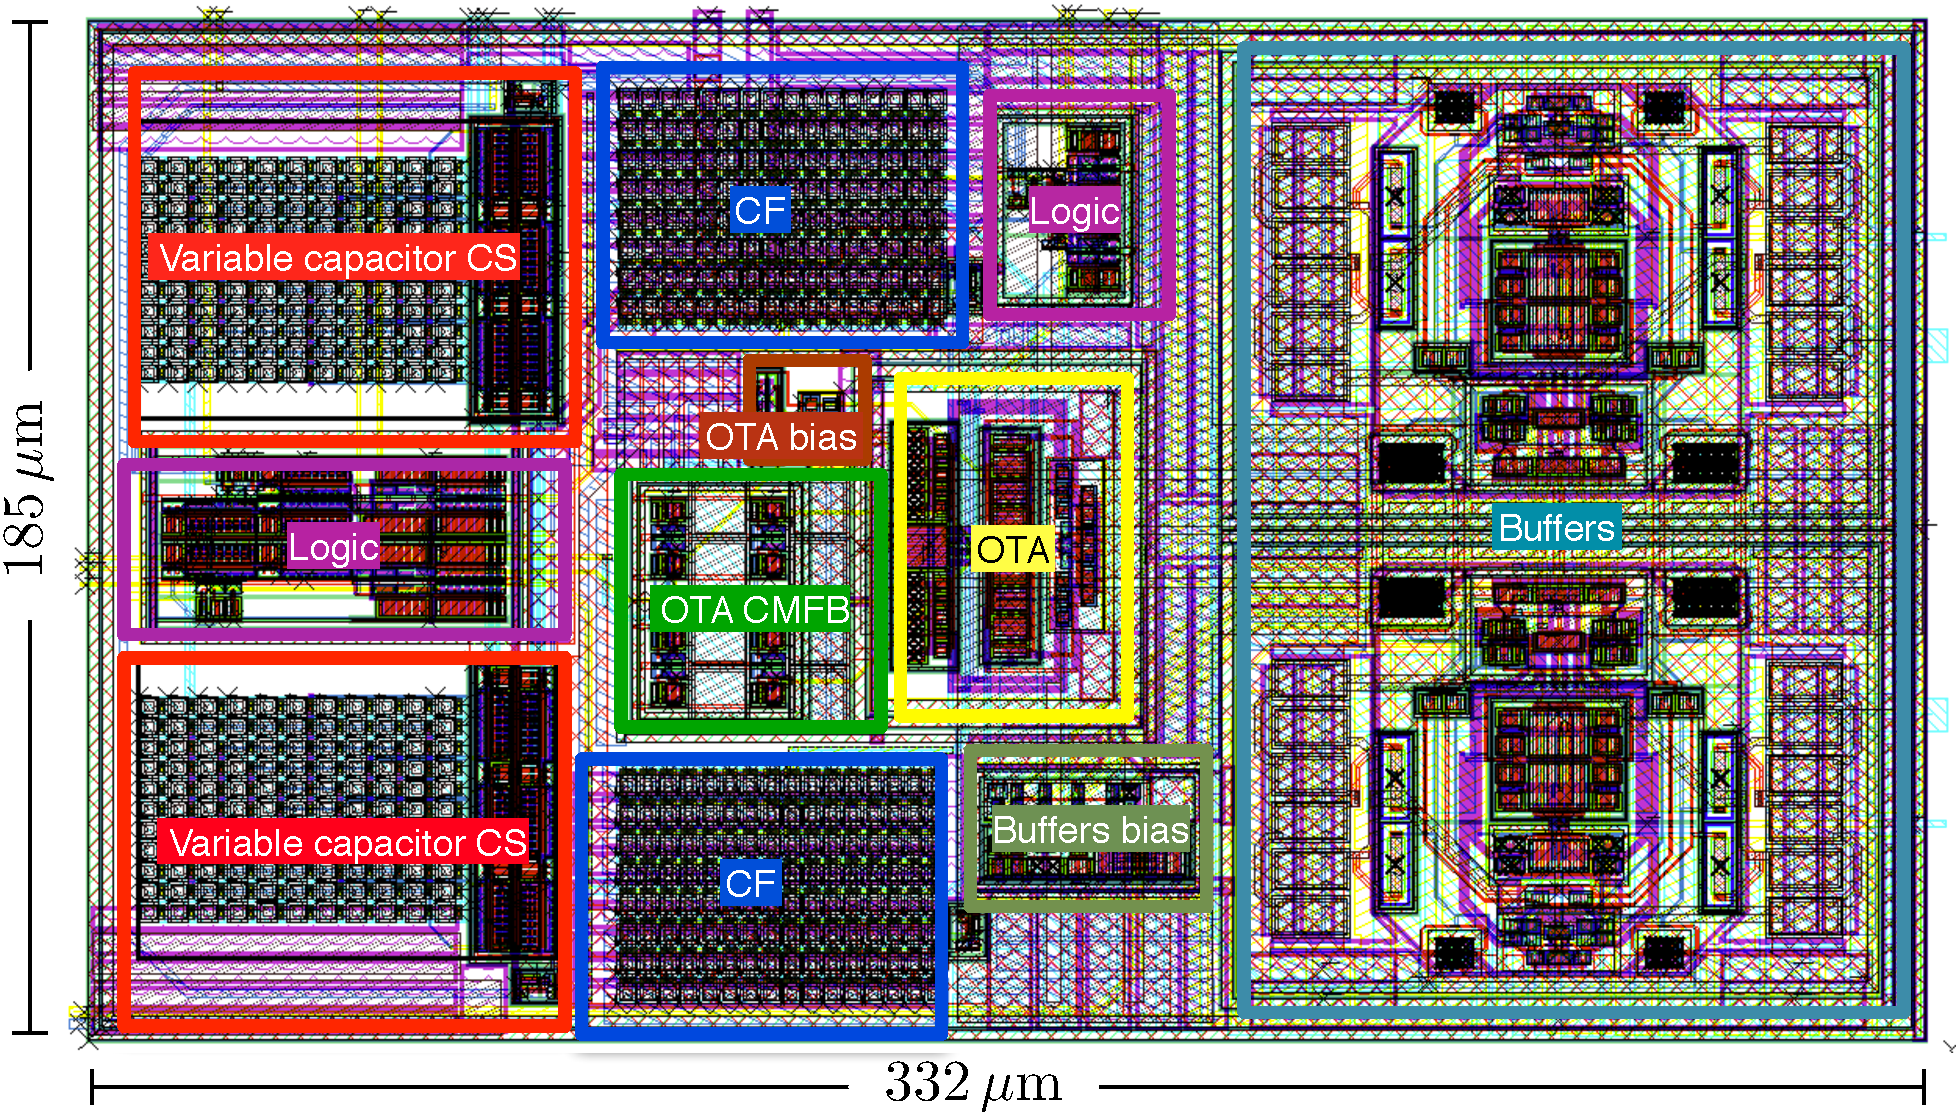
\includegraphics[width=6in]{./Figures/filter_layout}
	\caption{Filter Layout.}\label{fig:filter_layout}
\end{figure}


\begin{figure}[!p]
	\centering
	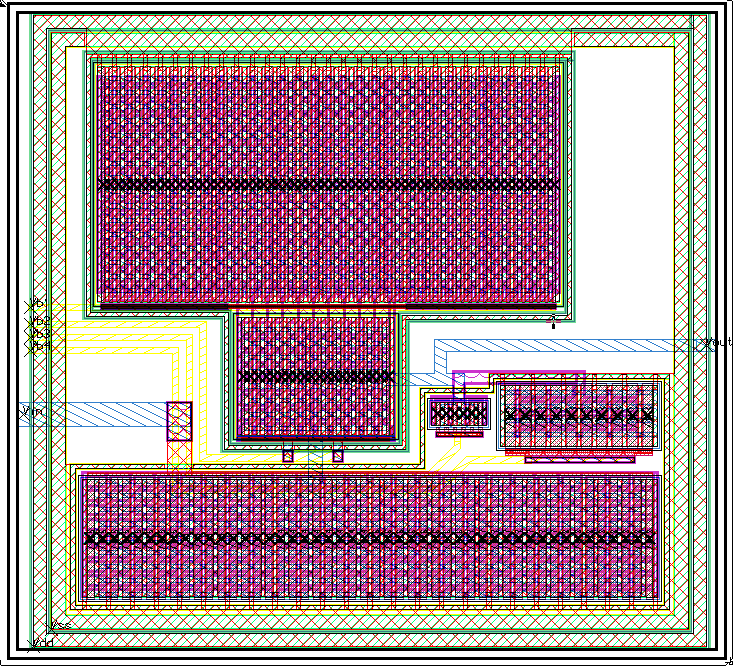
\includegraphics[width=4in]{./Figures/CSA_layout}
	\caption{Charge-sensitive amplifier layout. Feedback capacitors are not included here.}\label{fig:csa_layout}
\end{figure}

\begin{figure}[!t]
	\centering
	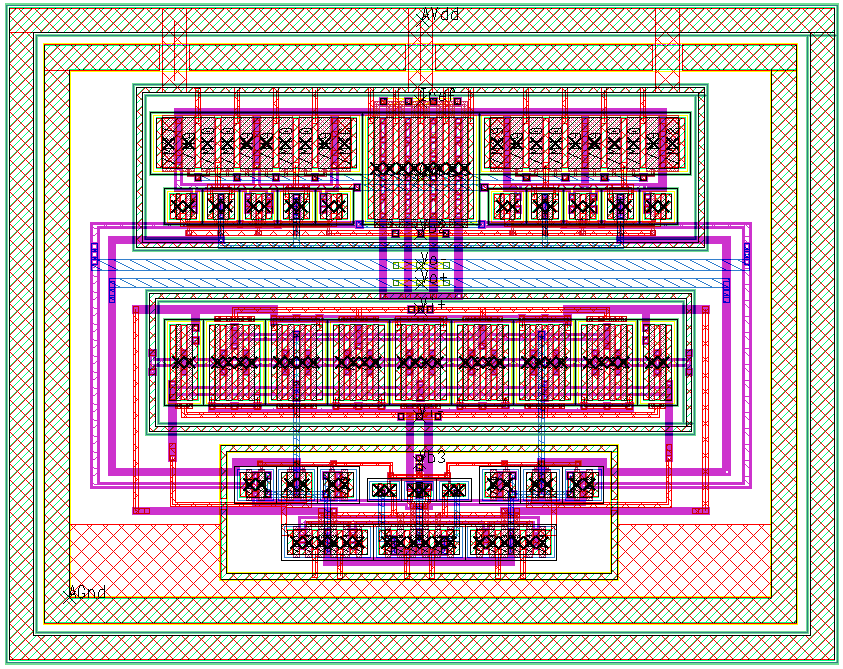
\includegraphics[width=4.5in]{./Figures/OTA_layout}
	\caption{Recycling folded cascode OTA layout.}\label{fig:ota_layout}
\end{figure}

\begin{figure}[!t]
	\centering
	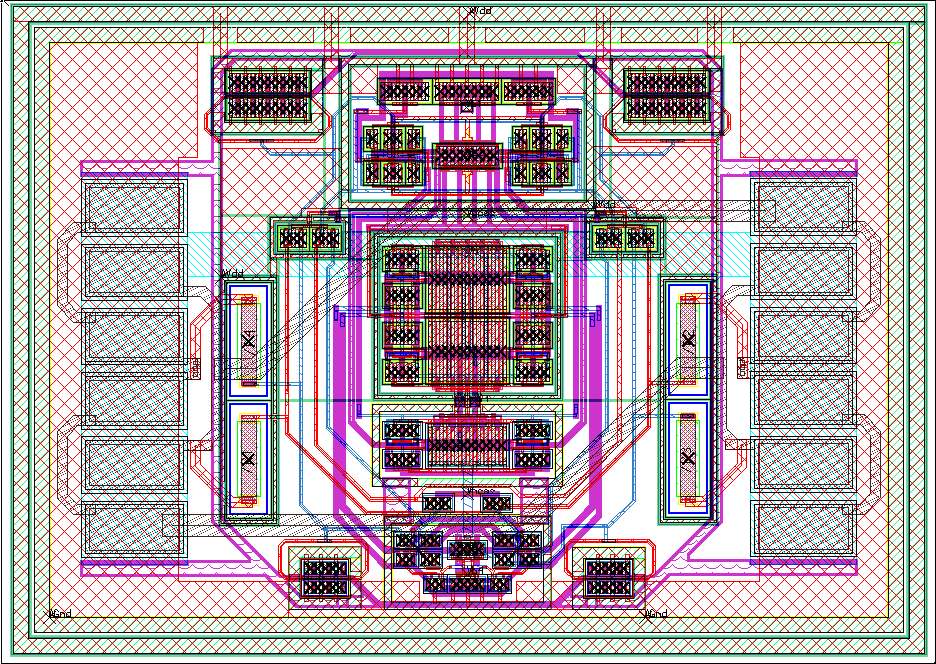
\includegraphics[width=4.5in]{./Figures/buffer_layout}
	\caption{Rail-to-rail operational amplifier layout.}\label{fig:buffer_layout}
\end{figure}

Because of the lack of models for the pads provided by Faraday and the tools needed to use them, it was necessary to design custom pads. They were designed for ground, positive supply voltage, analog input/output, digital input, and digital output. Special care was taken for the Latch-up failure of the output digital drivers, and the electrostatic discharge phenomena. 

\section{Filter post-layout simulation results}
\subsection{Sub-blocks}
The filter OTA and the buffer op-amp are the complex sub-blocks of the design. Thus, before proceeding with the complete layout, both structures were extracted separately and simulated individually. Figs.~\ref{fig:bode_OTA} and \ref{fig:bode_buffer}  shows the simulated open-loop response of the filter OTA and the buffer op-amp, respectively. The results are very close to the \mbox{pre-layout} simulation results of Chapter \ref{chapter:filter}, the most important difference is that the phase margin of the \mbox{op-amp} is $8^\circ$ lower than the pre-layout estimation. However, it is still within a safe and stable margin. To prove stability, exhaustive transients simulations were run using sharp voltage steps on the inputs, the power supply and the different voltage references. Special care was taken to prove stability of the $\beta$ multiplier circuit.

\begin{figure}[!t]
	\centering
	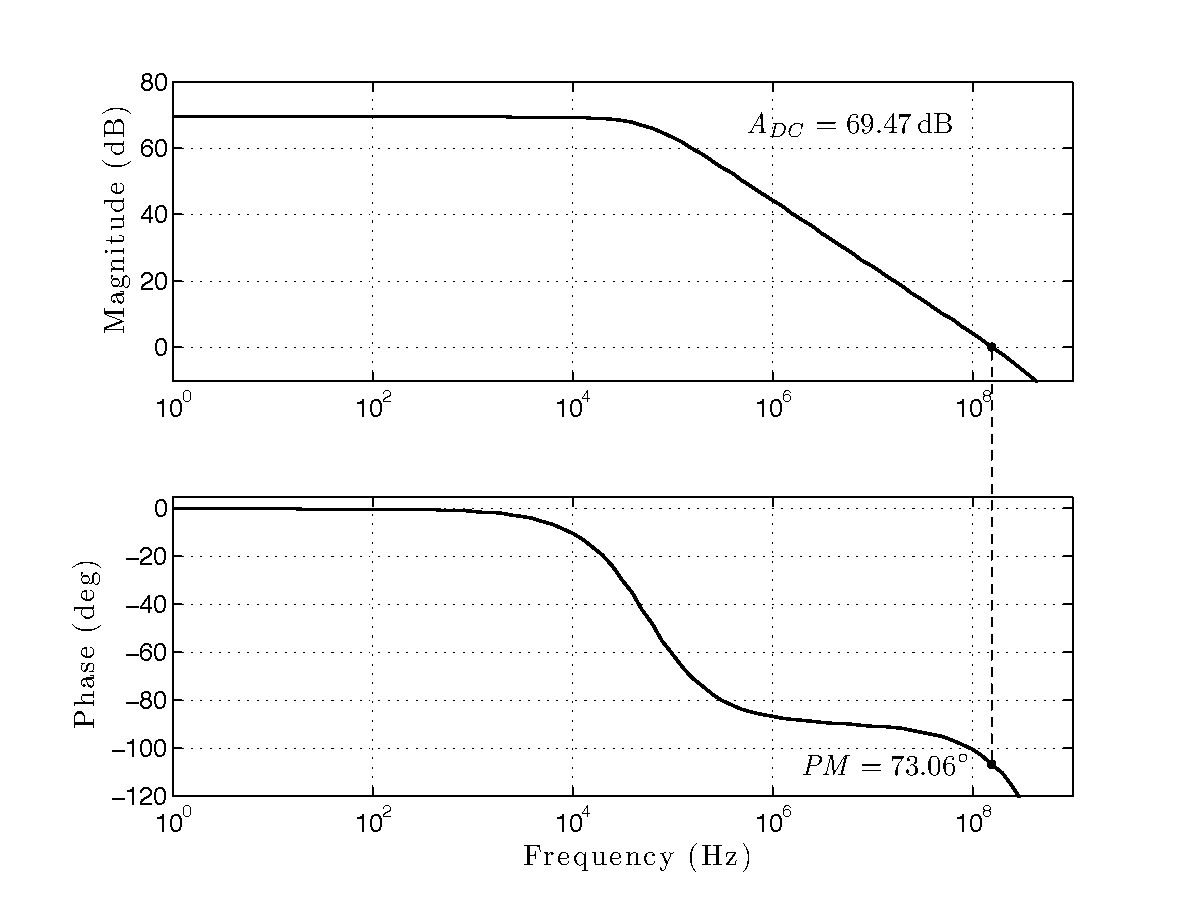
\includegraphics[width=5.3in]{./Test/bode_OTA_post}
	\caption{Bode plot for the OTA open-loop response, with a $0.4\,\text{pF}$ load capacitance.}\label{fig:bode_OTA}
\end{figure}

\begin{figure}[!t]
	\centering
	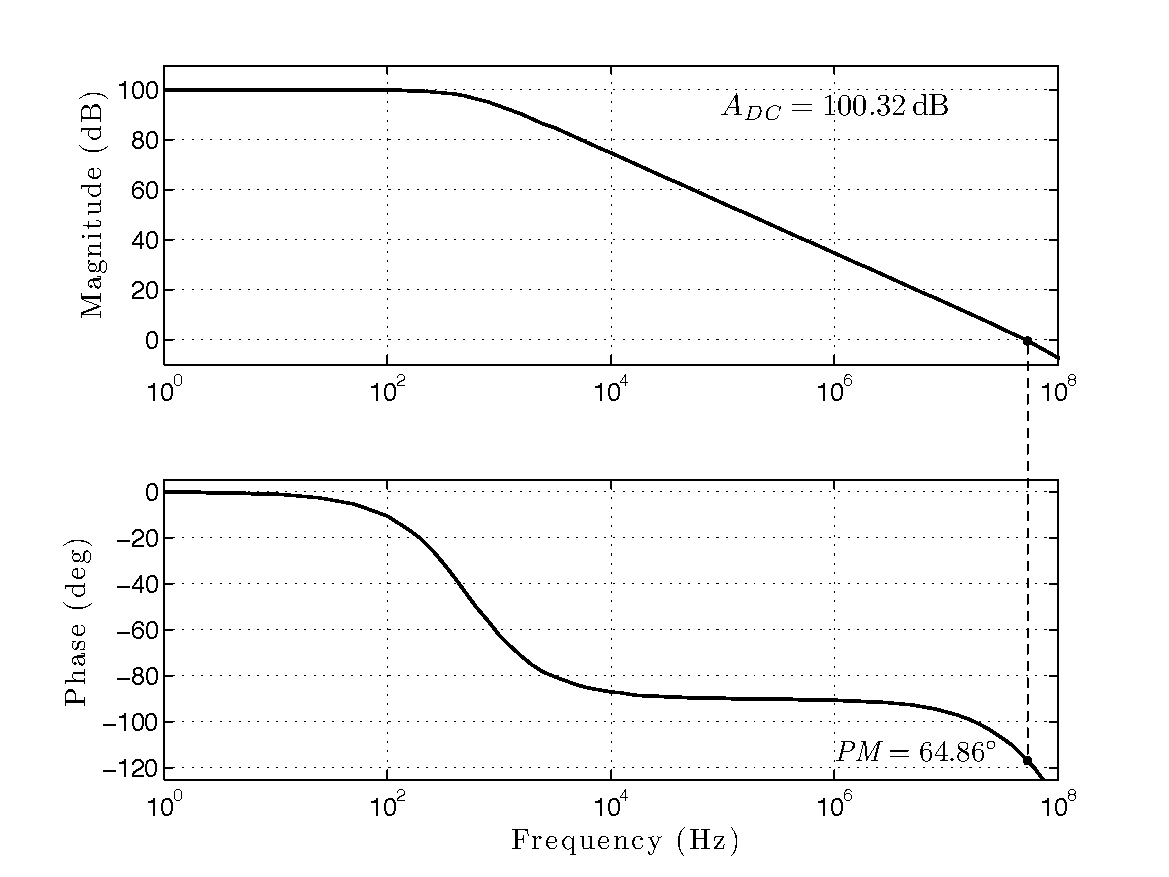
\includegraphics[width=5.3in]{./Test/bode_buffer_post}
	\caption{Bode plot for the buffer open-loop response, with a $8\,\text{pF}$ load capacitance.}\label{fig:bode_buffer}
\end{figure}

\subsection{Power dissipation} 

The power dissipated by the SC filter prototype was estimated using transient simulations over the extracted filter, under nominal operation and a single input value. The results are presented in Table~\ref{tab:power_dissipation}. The measurements are current consumption averages of the supply node of each component, thus, taking into account dynamic power consumption of the logic circuits.  

\begin{table}
	\begin{center}
		\begin{tabular}{|l|c|}\hline
			{\bf Component} & {\bf Current dissipation} \\ \hline\hline
			%CSA & $2.718\,\text{mW}$ \\ \hline			
			%CSA bias & $0.954\,\text{mW}$ \\ \hline			 
			Filter OTA & $369\,\mu\text{A}$ \\ \hline
			Filter bias and logic & $194\,\mu\text{A}$ \\ \hline
			Unity-gain buffer & $360\,\mu\text{A}$ \\ \hline
		\end{tabular}
		\vspace*{5pt}
		\caption{SC filter simulated current dissipation.}
		\label{tab:power_dissipation}
	\end{center}
\end{table}


\subsection{Functionality} 
A transient simulation using the entire extracted SC filter, including the bias structures, the buffers and the non-overlapping two-phase clock generator, was used to test the filter functionality. Control signals were driven with piecewise-linear voltage sources and a differential voltage step was used as filter input. Fig.~\ref{fig:test_filter_after_omni} shows the simulation result. The measured waveform confirms the functionality of all blocks.

A single clock cycle transient simulation was used to test the variable gain functionality of the filter. The control signals for the variable capacitors were driven with piecewise-linear voltage sources and a differential voltage step was used as filter input. Fig.~\ref{fig:gain_curves} shows the filter step response for the 64 available filter gains. The simulation confirms the monotonically increasing characteristic of the filter gain. However, the increments are not constant between consecutive filter gains. This can be explained due to the use of a binary array to implement the variable capacitor. This could be improved using a thermometer array or a mix between both, at the cost of adding complexity.

\begin{figure}[!t]
	\centering
	\includegraphics[width=5in]{./Test/test_filter_after_omni.eps}
	\caption{Filter functionality simulation. $V_\textit{in}=0.1\,V$ and $\text{gain}=0.25\,V/V$.}\label{fig:test_filter_after_omni}
\end{figure}

\begin{figure}[!t]
	\centering
	\includegraphics[width=4.4in]{./Test/gain_curves.pdf}
	\caption[Filter step response for constant input for the 64 possible programmable gains.]{Filter step response for constant input for the 64 possible programmable gains. \mbox{$V_\textit{in}=0.1\,V$} and \mbox{$T_s=40\,\text{ns}$}.}\label{fig:gain_curves}
\end{figure}

\subsection{Linearity}
The filter Integral nonlinearity (INL) was simulated for an input ramp covering $100\%$ of the filter input range. The simulations were carried out for nominal speed, with an input ramp driven by an ideal voltage source. Fig.~\ref{fig:inl} shows the simulation result. The INL plot shows a typical second order non-linear behavior caused by variations over the filter OTA gain due to the input range. This can be improved with a constant-$g_m$ OTA input stage and by increasing the OTA open-loop gain.  Spikes on the INL plot are caused by simulation numerical errors, thus they do not represent any filter dysfunction. The high value of the INL is due to the insufficient time for the filter to settle. Future revision of the Bean should consider the filter dynamical behavior and take special attention to the common-mode feedback loop, which was one of the factors that affected the filter settling time in this iteration of the design. 

\begin{figure}[!t]
	\centering
	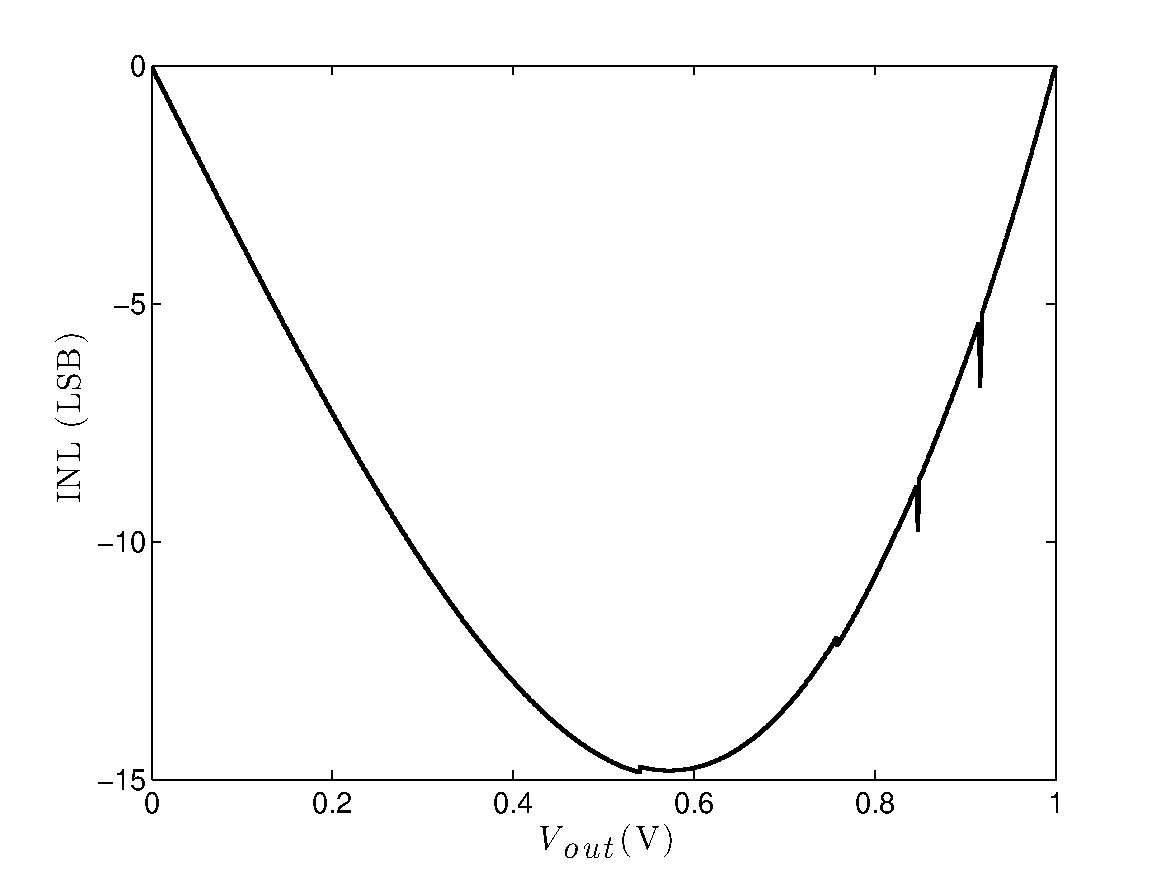
\includegraphics[width=4.4in]{./Test/linearity.pdf}
	\caption{Filter linearity simulation results, full-scale input range.}\label{fig:inl}
\end{figure}

\subsection{Weighting function}
The filter weighting function (WF) was simulated according to its definition described in Chapter~\ref{chapter:theoretical}. This was done by applying an input voltage step at different times within a cycle, and measuring the output at the measurement time. A simple $RC$ network was used to simulate a voltage step as seen at the output of a CSA. Fig.~\ref{fig:wf_test_circuit} shows the circuit used to perform this measurement. 

Fig.~\ref{fig:sim_wf} shows the post-layout SPICE-simulated WF of the filter using flat coefficients and the Bean nominal clock frequency. As expected, its shape resembles the shape of the WFs in Fig.~\ref{fig:optimum_wf},  which confirm the functionality of the filter to synthesize practical WFs. The initial non-zero value is caused by the successive integration of the filter input-referred offset voltage and the filter nonlinearities. Future revision of the filter could include a chopper-stabilized OTA to reduce the offset, and thus, to reduce the WF nonideality.

\begin{figure}[!t]
	\centering
	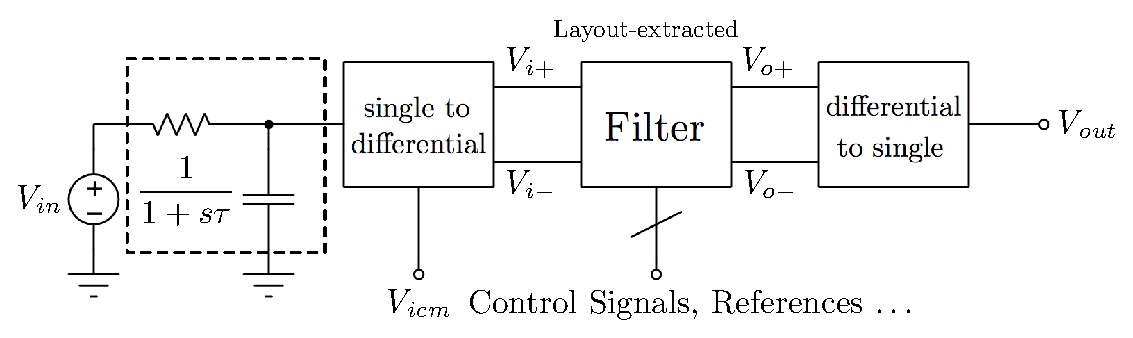
\includegraphics[width=5in]{./Test/wf_test_circuit}
	\caption{Weighting function test circuit.}\label{fig:wf_test_circuit}
\end{figure}

\begin{figure}[!t]
	\centering
	\includegraphics[width=3.6in]{./Test/sim_wf}
	\caption{SPICE-simulated weighting function. $\tau=8\,\text{ns}$, $N=16$ and $T_s=19.25\,\text{ns}$.}\label{fig:sim_wf}
\end{figure}









\clearpage
\chapter{CONCLUSION}
\label{chapter:conclusion}
\section{Summary}

This thesis deals with the use of discrete-time filters to process the noise present in particle physics detectors front-end circuits. The main contributions of this work are: the development of a new mathematical framework for a design-oriented analysis of \mbox{discrete-time} filters in the \mbox{discrete-time} domain; and the design and implementation of a switched capacitor (SC) filter for arbitrary weighting function (WF) synthesis to be included in the Bean V2 IC.

One of the most important topics in particle physics instrumentation is finding the optimal WF for noise minimization. Although some WFs, such as the cusp \citep{radeka104}, are impossible to synthesize using continuous-time circuits, it was then interesting to determine the fundamental lower limit of noise that could be achieved through them. From then on, design efforts were focused on synthesizing the closest WFs to these theoretical optimal ones. Once introduced the discrete-time pulse shapers in the early 90's, the design efforts remained on this path, by using discrete-time filters to synthesize WFs similar to the continuous-time optimal WFs. However, this approach ignores the discrete-time nature of the pulse shaper, since taking into account this condition results in different optimal WFs, which for a variety of conditions could be very different to the continuos-time counterparts.  This problem leads to the main work presented in this thesis, a mathematical framework to calculate the noise of a typical detector front-end circuit from a \mbox{discrete-time} point of view, and thereby, a powerful tool to design the optimal discrete-time pulse shapers.

From a practical point of view, a generic filter for arbitrary weighting function synthesis is an ideal companion for the theoretical framework mentioned above. The design of this filter was presented in this work, framed on the design of the Bean V2,  an application specific integrated circuit (ASIC) planned to meet the BeamCal instrumentation needs. The use of this filter,  along with a proper characterization of the CSA and detector noise statistics, will allow to minimize the output referred noise on the BeamCal front-end circuit.

\section{Future work}

The mathematical framework presented in this work depends on a proper characterization of the CSA and detector noise statistics to find the optimal filter. Once estimated these parameters, the filter coefficients are computed offline, and then, they are updated in the circuit. An interesting future development could be to find a methodology to compute the filter coefficients online without having to characterize the CSA and detector noise statistics separately. To pursue this problem, the mathematical framework presented in this work represents a proper starting point. Also, given the abstraction of this work, it could find applications in other fields with similar circuit configurations, such as the current developments for astronomical instrumentation \citep{guzman101}.

The lessons learned during the design and simulation of the Bean filter prototype will prompt corrections, improvements, and upgrades for future revisions. Based just on simulation results, the most urgent correction consist of editing the filter OTA design to meet the settling time specification, and thus, the linearity specification.  Filter lab testing are about to start. Additional corrections, improvements, and upgrades are expected as result of this development phase.


% References



%%%%%%%%%%%%%%%%%%%%%%%%%%%%%%%%%%%%%%%%%%%%%%%%%%%%%%%%%%%%%%%%%%%%%%%%
% Begin Appendix



\cleardoublepage
\bibliographystyle{apacite}
\bibliography{\bibpath/library}
\cleardoublepage

\cleardoublepage
\thispagestyle{empty}
\begin{center}
\vspace*{3.5in}
\large{\bfseries{APPENDIX}}
\addcontentsline{toc}{chapter}{APPENDIX}
\end{center}

\appendix
\cleardoublepage


\chapter{Anexos}
\section{Pinout de the Bean V2}
 \label{appendix1}
El prototipo de The Bean V2 tiene 48 pads y fue bonded a 64-lead package from \mbox{Kyocera} Corporation (KYO). The package KYO part number is QC064307WZ. Table \ref{pinout} shows the Bean V2 pinout.


\begin{center}
\begin{longtable}{|l|l|l|}\hline
{\bf Pin number} & {\bf Pin name} & {\bf Description} \\ \hline\hline
1 & \verb=AGnd= & Analog ground \\\hline
2 & \verb=NC= & No connection \\\hline
3 & \verb=NC= & No connection \\\hline
4 & \verb=NC= & No connection \\\hline
5 & \verb=NC= & No connection \\\hline
6 & \verb=res_bias_ext= & IC bias external resistor \\\hline
7 & \verb=V_ref_prechar= & Reference voltage CSA precharger \\\hline
8 & \verb=NC= & No connection  \\\hline
9 &  \verb=clk_prech1= & CSA precharger clk1  \\\hline
10 & \verb=clk_prech2= & CSA precharger clk2  \\\hline
11 & \verb=op_mode= & Operation mode select \\\hline
12 & \verb=rst_csa= & CSA reset  \\\hline
13 & \verb=NC= & No connection \\\hline
14 & \verb=cap_precharge_ext= & CSA precharger external capacitor \\\hline
15 & \verb=Vin_csa= & Vin CSA \\\hline
16 & \verb=AGnd= & Analog ground \\\hline
17 & \verb=AGnd= & Analog ground \\\hline
18 & \verb=NC= & No connection \\\hline
19 & \verb=NC= & No connection \\\hline
20 & \verb=clk= & IC clock \\\hline
21 & \verb=NC= & No connection \\\hline
{\bf Pin number} & {\bf Pin name} & {\bf Description} \\ \hline\hline
22 & \verb=Vi+_fil= & Filter Vi+ \\\hline
23 & \verb=Vi-_fil= & Filter Vi- \\\hline
24 & \verb=Vo+_bp_fil= & Filter bypass Vo+  \\\hline
25 & \verb=Vo-_bp_fil= & Filter bypass Vo- \\\hline
26 & \verb=NC= & No connection \\\hline
27 & \verb=DVdd= & Digital Vdd \\\hline
28 & \verb=DGnd= & Digital Gnd \\\hline
29 & \verb=NC= & No connection \\\hline
30 & \verb=Vo+_fil= & Filter Vo+ (buffered) \\\hline
31 & \verb=Vo-_fil= & Filter Vo- (buffered) \\\hline
32 & \verb=AGnd= & Analog ground \\\hline
33 & \verb=AGnd= & Analog ground \\\hline
34 & \verb=NC= & No connection \\\hline
35 & \verb=out_s= & Filter output selection \\\hline
36 & \verb=Vocm= & Filter Vocm \\\hline
37 & \verb=hold= & Filter hold signal  \\\hline
38 & \verb=rst= & Filter reset \\\hline
39 & \verb=sgn= & Filter gain sign \\\hline
40 & \verb=Vicm= & Filter Vicm \\\hline
41 & \verb=CS_b0= & Filter CS capacitor bit 0 \\\hline
42 & \verb=CS_b1= & Filter CS capacitor bit 1 \\\hline
43 & \verb=CS_b2= & Filter CS capacitor bit 2 \\\hline
44 & \verb=CS_b3= & Filter CS capacitor bit 3 \\\hline
45 & \verb=CS_b4= & Filter CS capacitor bit 4 \\\hline
46 & \verb=CS_b5= & Filter CS capacitor bit 5 \\\hline
47 & \verb=NC= & No connection \\\hline
{\bf Pin number} & {\bf Pin name} & {\bf Description} \\ \hline\hline
48 & \verb=AGnd= & Analog ground \\\hline
49 & \verb=AGnd= & Analog ground \\\hline
50 & \verb=Vo+_ch= & Channel Vo+ (buffered) \\\hline
51 & \verb=NC= & No connection \\\hline
52 & \verb=Vo-_ch= & Channel Vo- (buffered)\\\hline
53 & \verb=NC= & No connection \\\hline
54 & \verb=Vout_csa= & CSA Vout (buffered) \\\hline
55 & \verb=NC= & No connection \\\hline
56 & \verb=baseline= & CSA baseline (buffered) \\\hline
57 & \verb=NC= & No connection \\\hline
58 & \verb=AGnd= & Analog ground \\\hline
59 & \verb=NC= & No connection \\\hline
60 & \verb=NC= & No connection \\\hline
61 & \verb=NC= & No connection \\\hline
62 & \verb=AVdd= & Analog Vdd \\\hline
63 & \verb=NC= & No connection \\\hline
64 & \verb=AGnd= & Analog ground \\\hline
\caption{\label{pinout}The Bean 2 prototype pinout}
\end{longtable}
\end{center}












\clearpage
\begin{center}
\begin{longtable}{|l|l|l|l|}\hline
{\bf Nombre} & {\bf FX02} & {\bf Verilog}&{\bf Módulo} \\ \hline\hline
\verb=CLK_DAC= &A16&\verb+PIO10+& \verb+DAC_CTRL+ \\\hline
\verb=SDI_DAC= &A15&\verb+PIO9+& \verb+DAC_CTRL+ \\\hline
\verb=CLK_DAC= &A14&\verb+PIO8+& \verb+DAC_CTRL+ \\\hline
\verb=SDI_REF= &A6&\verb+PIO0+& \verb+DigiPot_CTRL+ \\\hline
\verb=CLK_REF= &A8&\verb+PIO2+& \verb+DigiPot_CTRL+ \\\hline
\verb=CS1_REF= &A11&\verb+PIO5+& \verb+DigiPot_CTRL+ \\\hline
\verb=CS2_REF= &A10&\verb+PIO4+& \verb+DigiPot_CTRL+ \\\hline
\verb=CS3_REF= &A7&\verb+PIO1+& \verb+DigiPot_CTRL+ \\\hline
\verb=MUX1_REF= &A12&\verb+PIO6+& \verb+MUX_CTRL+ \\\hline
\verb=MUX2_REF= &A13&\verb+PIO7+& \verb+MUX_CTRL+ \\\hline
\verb=MUX3_REF= &A9&\verb+PIO3+& \verb+MUX_CTRL+ \\\hline
\verb=MUX_DAC_EN= &A22&\verb+PIO16+& \verb+MUX_CTRL+ \\\hline
\verb=SDO_ADC2= &A18&\verb+PIO12+& \verb+ADC2_CTRL+ \\\hline
\verb=CS_ADC2= &A19&\verb+PIO13+& \verb+ADC2_CTRL+ \\\hline
\verb=CLK_ADC2= &A20&\verb+PIO14+& \verb+ADC2_CTRL+ \\\hline
\verb=SDO_ADC1= &A43&\verb+PIO37+& \verb+ADC1_CTRL+ \\\hline
\verb=CS_ADC1= &A44&\verb+PIO38+& \verb+ADC1_CTRL+ \\\hline
\verb=CLK_ADC1= &A45&\verb+PIO39+& \verb+ADC1_CTRL+ \\\hline
\verb=out_s= &A24&\verb+PIO18+& the\_bean\_config \\\hline
\verb=hold= &A25&\verb+PIO19+& the\_bean\_config \\\hline
\verb=rst= &A26&\verb+PIO20+& the\_bean\_config \\\hline
\verb=sgn= &A27&\verb+PIO21+& the\_bean\_config \\\hline
\verb=CS_B0= &A28&\verb+PIO22+& the\_bean\_config \\\hline
\verb=CS_B1= &A30&\verb+PIO24+& the\_bean\_config \\\hline
\verb=CS_B2= &A32&\verb+PIO26+& the\_bean\_config \\\hline
\verb=clk= &A33&\verb+PIO27+& the\_bean\_config \\\hline
{\bf Nombre} & {\bf FX02} & {\bf Verilog}&{\bf Módulo} \\ \hline\hline
\verb=CS_B3= &A34&\verb+PIO28+& the\_bean\_config \\\hline
\verb=rst_csa= &A35&\verb+PIO29+& the\_bean\_config \\\hline
\verb=CS_B4= &A36&\verb+PIO30+& the\_bean\_config \\\hline
\verb=op_mode= &A37&\verb+PIO31+& the\_bean\_config \\\hline
\verb=CS_B5= &A38&\verb+PIO32+& the\_bean\_config \\\hline
\verb=clk_pc_1= &A40&\verb+PIO34+& the\_bean\_config \\\hline
\verb=clk_pc_2= &A42&\verb+PIO36+& the\_bean\_config \\\hline
\verb=MUX_DAC_SEL= &A21&\verb+PIO15+& the\_bean\_config \\\hline
\caption{\label{pinout2}Lista de distribución de pines para el controlador de la tarjeta.}
\end{longtable}
\end{center}



\begin{figure}[!t]
	\centering
	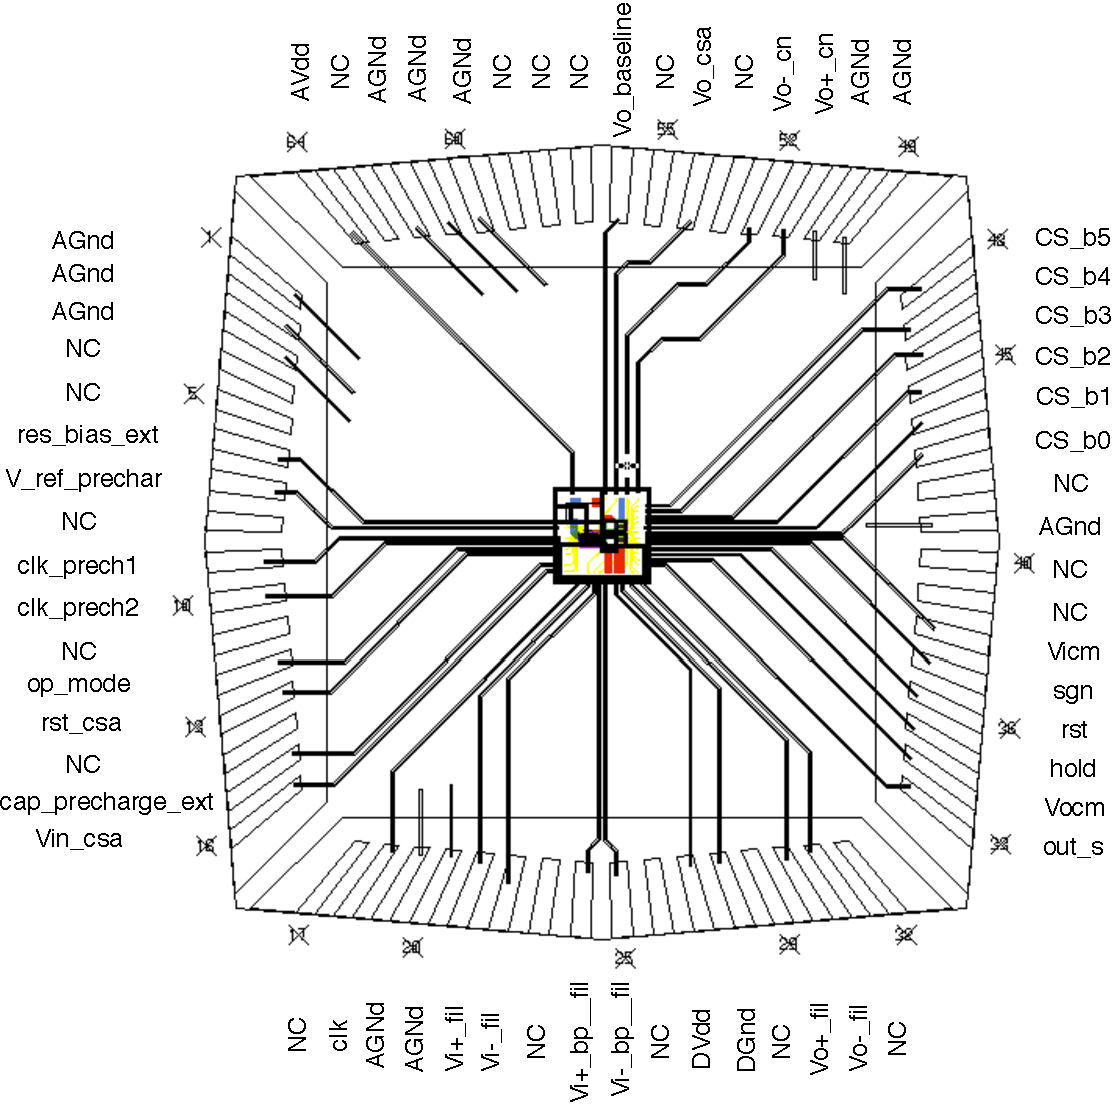
\includegraphics[width=6in]{./Figures/bondpad.pdf}
	\caption{The Bean 2 prototype bonding diagram.}\label{fig:bondpad}
\end{figure}



\end{document}


